
\documentclass[a4paper,spanish,11pt]{article}

\usepackage[utf8]{inputenc}
\usepackage[spanish]{babel}
\usepackage{fontenc}
\usepackage{amssymb}
\usepackage{color}
\usepackage{graphics}
\usepackage{listings}
\usepackage{moreverb}             % Para que separe bien las sílabas
\usepackage{caratula} 
\usepackage{a4wide}
\usepackage{fancyhdr}
\usepackage{multirow}
\usepackage{booktabs}
\usepackage{pdfpages}
\usepackage{amsmath}
\lstset{                % general command to set parameter(s)
 language=C,
 basicstyle=\small,      % print whole listing small
 keywordstyle=\bfseries, % underlined bold black keywords
 stringstyle=\ttfamily, % typewriter type for strings
 showstringspaces=false
} 
\lstset{
 numbers=left, 
 numberstyle=\tiny, 
 stepnumber=5,
 numbersep=5pt}	


 \newcommand{\integranteuno}{Castro - }
 
 \newcommand{\materiaP}{Investigación Operativa} 
 \newcommand{\tituloTP}{Trabajo Práctico} 
 \newcommand{\subTituloTP}{} 
 %\newcommand{\cuatHEADER}{2C 2008}

\pagestyle{fancyplain} 

\begin{document}

\titulo{\tituloTP}
\fecha{\today}
\materia{\materiaP}
%\grupo{Nombre Grupo}
\integrante{Castro, Sabrina Elizabeth}{572/01}{sabrinaecastro@gmail.com}

\maketitle


\fancyhf{} %borra 
 \setcounter{page}{1}%que el contador empiece de uno con la primer pagina, no con la caratula
\lhead[\materiaP]{\materiaP}
% \rhead[\cuatHEADER]{\cuatHEADER}
 
 \lfoot[\subTituloTP]{\integranteuno \tituloTP}
 \rfoot[{\thepage}]{{\thepage}}


%\begin{abstract}

 
%\end{abstract}
\newpage
\tableofcontents
\newpage
%\section{Introducci\'on}
%     

%    \newpage
    \section{Fabricación de alimentos}
\subsection{Enunciado 12-1} 
\paragraph{}Un alimento se fabrica refinando aceites crudos y mezclandolos. Los aceites crudos son de dos categorias:
\begin{center}
\begin{tabular}{@{}cl@{}}
\hline
\multirow{2}{*}{\begin{tabular}[c]{@{}c@{}}Aceites vegetales\end{tabular}}     & Veg 1 \\
                                                                                  & Veg 2 \\
\multirow{3}{*}{\begin{tabular}[c]{@{}c@{}}Aceites no vegetabes\end{tabular}} & Oil 1 \\
                                                                                  & Oil 2 \\
                                                                                 & Oil 3\\
                                                                                 \hline 
\end{tabular}
\end{center}
\paragraph{}Cada aceite puede comprarse para entrega inmediata (enero) o comprarse en el mercado para una entrega futura en un mes posterior. Los precios se indican a continuacion(\pounds /ton):\\

\begin{center}
\begin{tabular}{|c|c|c|c|c|c|}
\hline 
 & Veg 1 & Veg 2 & Oil 1 & Oil 2 & Oil 3 \\ 
\hline 
Enero & 110 & 120 & 130 & 110 & 115 \\ 
\hline 
Febrero & 130 & 130 & 110 & 90 & 115 \\ 
\hline 
Marzo & 110 & 140 & 130 & 100 & 95 \\ 
\hline 
Abril & 120 & 110 & 120 & 120 & 125 \\ 
\hline 
Mayo & 100 & 120 & 150 & 110 & 105 \\ 
\hline 
Junio & 90 & 100 & 140 & 80 & 135 \\ 
\hline 
\end{tabular} 
\end{center}

\paragraph{}El producto final se vende a \pounds 150 por tonelada.
\paragraph{}Los aceites vegetales y los aceites no vegetales requieren diferentes lineas de producción para refinar. En cualquier mes, no es posible refinar mas de 200 toneladas de aceites vegetales y mas de 250 toneladas de aceites no vegetales. No hay perdida de peso en el proceso de refinación y el costo de refinacion puede ser ignorado.
\paragraph{}Es posible almacenar hasta 1000 toneladas de cada aceite crudo para su uso posterior. El costo de almacenamiento para el aceite vegetal y no vegetal es de \pounds 25 por tonelada por mes. El producto final no se puede almacenar, ni se pueden almacenar aceites refinados.
\paragraph{}Hay una restricción tecnologica de dureza en el producto final. En las unidades de las que se mide la dureza, esta debe estar entre 3 y 6. Se supone que la dureza se combina linealmente y que las durezas de los aceites crudos son:\\
\begin{center}
\begin{tabular}{|c|c|}
\hline 
Veg 1 & 8.8 \\ 
\hline 
Veg 2 & 6.1 \\ 
\hline 
Oil 1 & 2.0 \\ 
\hline 
Oil 2 & 4.2 \\ 
\hline 
Oil 3 & 5.0 \\ 
\hline 
\end{tabular} 
\end{center}

\paragraph{}¿Que políticas de compras y fabricación debería seguir la empresa para maximizar los beneficios?  
\paragraph{}En la actualidad hay 500 toneladas de cada tipo de aceite crudo almacenado. Se requiere que estas existencias también existan a fines de junio.

\subsection{Modelo}
$\begin{array}{l}
Cv_{i,j}: \mbox{cantidad de toneladas de aceite vegetal crudo VEG i comprado en el mes j}\\
Co_{t,j}: \mbox{cantidad de toneladas de aceite no vegetal crudo OIL t comprado en el mes j}\\
Rv_{i,j}: \mbox{cantidad de toneladas de aceite vegetal crudo VEG i refinado en el mes j}\\
Ro_{t,j}: \mbox{cantidad de toneladas de aceite no vegetal crudo IOL t refinado en el mes j}\\
Av_{i,j}: \mbox{cantidad de toneladas de aceite vegetal crudo VEG i almacenado en el mes j}\\
Ao_{t,j}: \mbox{cantidad de toneladas de aceite no vegetal crudo IOL t almacenado en el mes j}\\
i=1,2  \;\;\;\;\;\; t=1,2,3 \;\;\;\;\;\; j=1,2,3,4,5,6\\ \\
\mbox{donde j representa los meses }1 \mbox{ es enero}, 2 \mbox{ es febrero, y asi.}
\end{array} $
\\ \\ 
$$\ \mbox{maxizar   } 150\left( \sum_{j=1}^{6}Rv_{1,j}+Rv_{2,j}+Ro_{1,j}+Ro_{2,j}+Ro_{3,j}\right) $$
$$\ - 25\left( \sum_{j=1}^{6}Av_{1,j}+Av_{2,j}+Ao_{1,j}+Ao_{2,j}+Ao_{3,j}\right) $$
$$\ - \left( 110Cv_{1,1}+130Cv_{1,2}+110Cv_{1,3}+120Cv_{1,4}+100Cv_{1,5}+90Cv_{1,6}\right) $$
$$\ - \left( 120Cv_{2,1}+130Cv_{2,2}+140Cv_{2,3}+110Cv_{2,4}+120Cv_{2,5}+100Cv_{2,6}\right) $$
$$\ - \left( 130Co_{1,1}+110Co_{1,2}+130Co_{1,3}+120Co_{1,4}+150Co_{1,5}+140Co_{1,6}\right) $$
$$\ - \left( 110Co_{2,1}+90Co_{2,2}+100Co_{1,3}+120Co_{1,4}+110Co_{1,5}+80Co_{1,6}\right) $$
$$\ - \left( 115Co_{3,1}+115Co_{3,2}+95Co_{1,3}+125Co_{1,4}+105Co_{1,5}+135Co_{1,6}\right) $$
\\ \\ 
s.a\\
No se pude refinar mas de 200 toneladas de aceite vegetales
\begin{equation}
Rv_{1,j} + Rv_{2,j} \leq 200 
\end{equation}
No se pude refinar mas de 250 toneladas de aceite no vegetales
\begin{equation}
Ro_{1,j} + Ro_{2,j} + Ro_{3,j} \leq 250 
\end{equation}
No se puede almacenar mas de 1000 toneledas de aceite vegetal
\begin{equation}
Av_{i,j} \leq 1000
\end{equation}
No se puede almacenar mas de 1000 toneledas de aceite no vegetal
\begin{equation}
Ao_{t,j} \leq 1000
\end{equation}
La dureza en el producto final debe ser mayor que 3 y menor que 6
\begin{equation}
 \frac{ 8.8 Rv_{1,j} + 6.1 Rv_{2,j} + 2.0 Ro_{1,j} + 4.2 Ro_{2,j} + 5.0 Ro_{3,j} } { Rv_{1,j} + Rv_{2,j} + Ro_{1,j} + Ro_{2,j} + Ro_{3,j}} \geq 3
\end{equation}
\begin{equation}
 \frac{8.8 Rv_{1,j} + 6.1 Rv_{2,j} + 2.0 Ro_{1,j} + 4.2 Ro_{2,j} + 5.0 Ro_{3,j}}{Rv_{1,j} + Rv_{2,j} + Ro_{1,j} + Ro_{2,j} + Ro_{3,j}} \leq 6
\end{equation}
Lo comprado + lo almacenado - lo refinado en el mes j, es lo almacenado para el mes j+1, para j=1,2,3,4,5
\begin{equation}
Cv_{i,j} + Av_{i,j} - Rv_{i,j} = Av_{i,j+1}
\end{equation}
\begin{equation}
Co_{t,j} + Ao_{t,j} - Ro_{t,j} = Ao_{t,j} 
\end{equation}
Lo comprado + lo almacenado - lo refinado en el mes de junio, es lo almacenado despues de junio
\begin{equation}
Cv_{i,6} + Av_{i,6} - Rv_{i,6} = Av_{i,7}
\end{equation}
\begin{equation}
Co_{t,6} + Ao_{t,6} - Ro_{t,6} = Ao_{t,7} 
\end{equation}
En enero se comienza con 500 toneladas de cada aceite almacenado y se quiere terminar junio con la misma cantidad
\begin{equation}
Av_{1,1}=500
\end{equation}
\begin{equation}
Av_{2,1}=500
\end{equation}
\begin{equation}
Ao_{1,1}=500
\end{equation}
\begin{equation}
Ao_{2,1}=500
\end{equation}
\begin{equation}
Ao_{3,1}=500
\end{equation}
\begin{equation}
Av_{1,7}=500
\end{equation}
\begin{equation}
Av_{2,7}=500
\end{equation}
\begin{equation}
Ao_{1,7}=500
\end{equation}
\begin{equation}
Ao_{2,7}=500
\end{equation}
\begin{equation}
Ao_{3,7}=500
\end{equation}

\subsection{Modelo CPLEX}
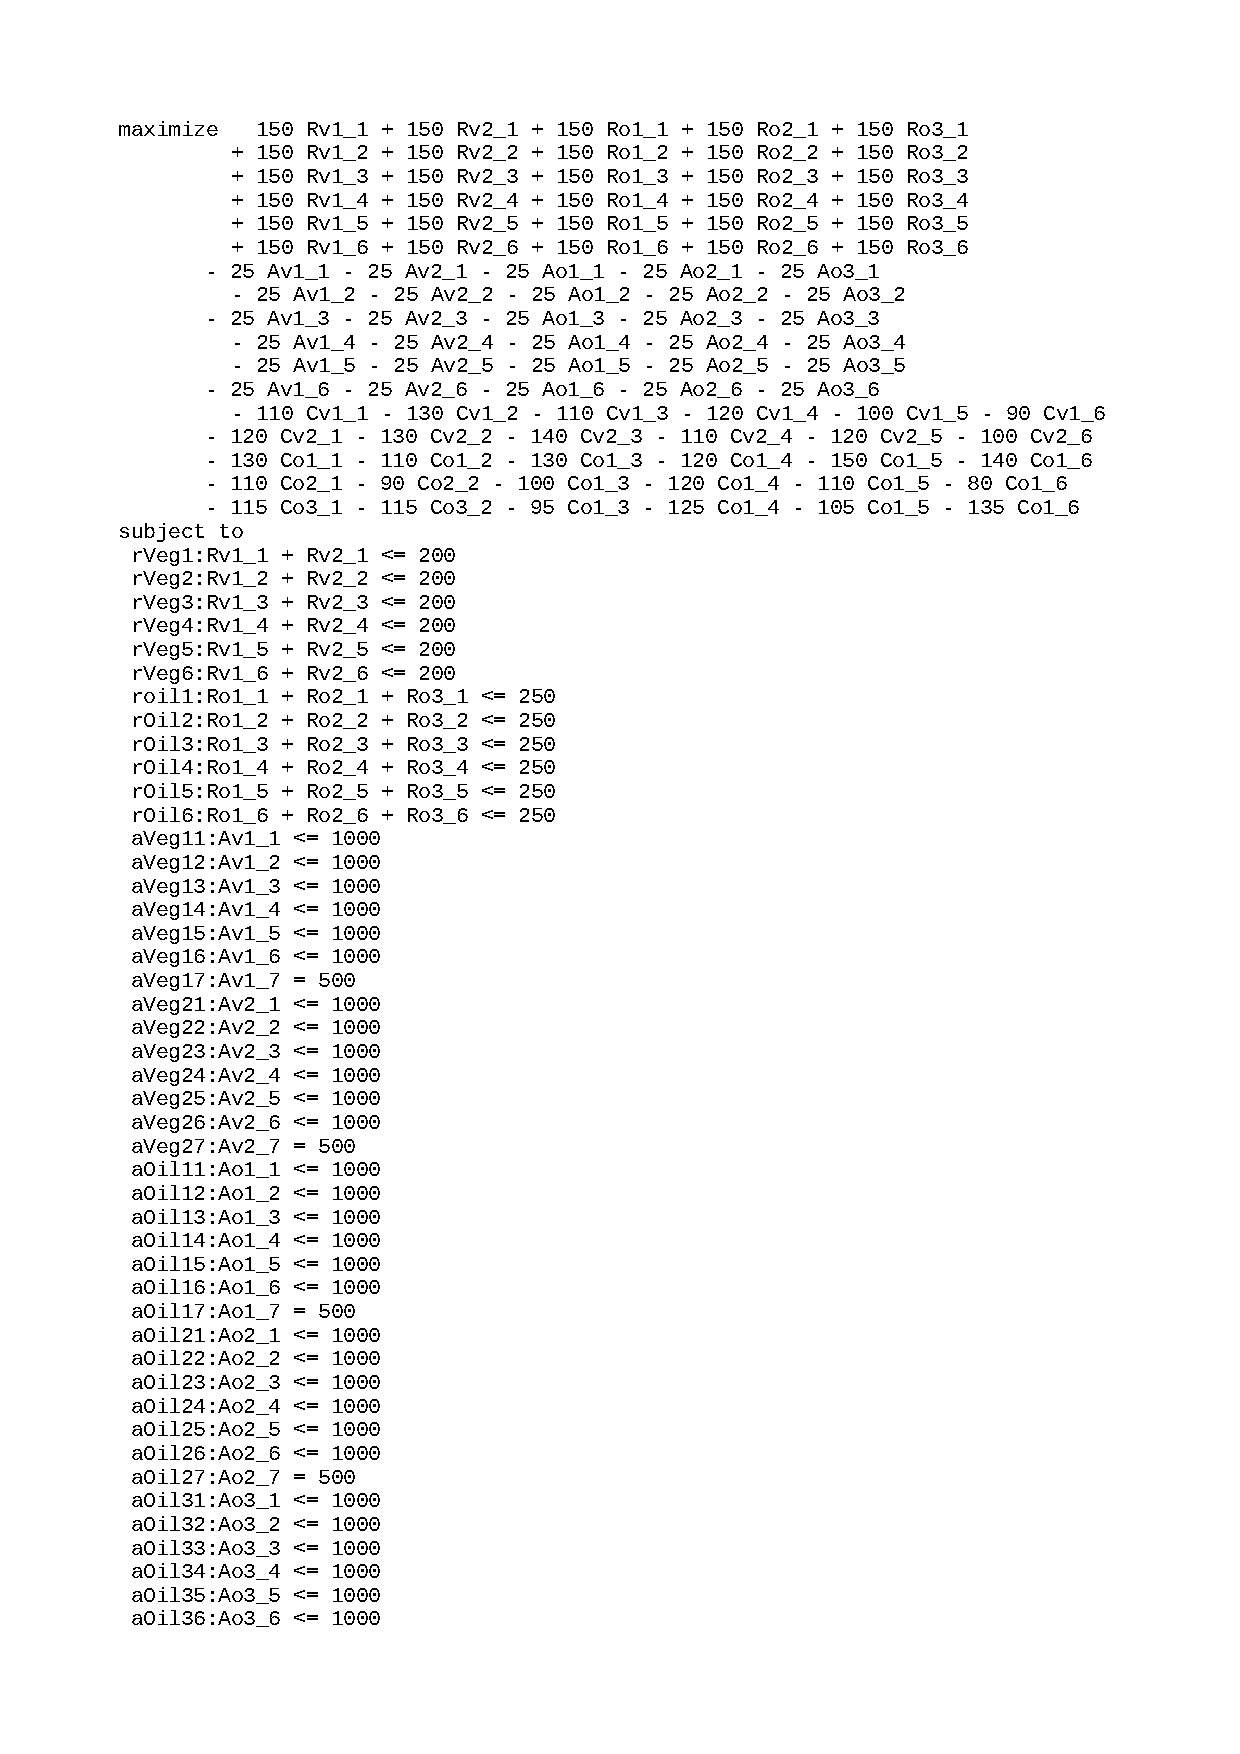
\includepdf[pages=1-2]{modelos/fabricaAlimentos12-1}


\subsection{Solucion CPLEX}
\paragraph{}¿Que políticas de compras y fabricación debería seguir la empresa para maximizar los beneficios?  

\begin{figure}[!h]
    \centering
    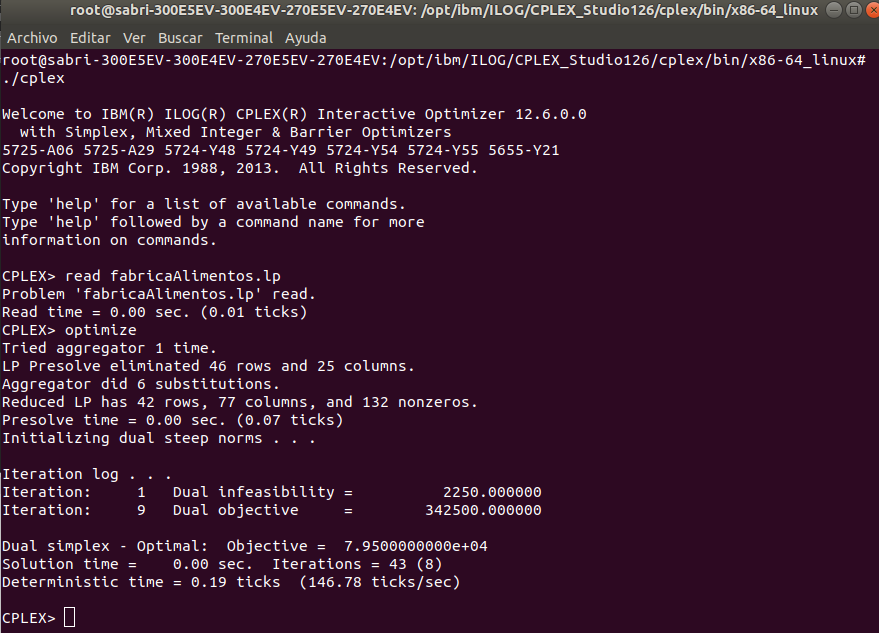
\includegraphics[scale=0.35]{modelos/fabricaAlimentos12-1Solucion.png}
    \caption{Solución}
\end{figure}

\begin{figure}[!h]
    \centering
    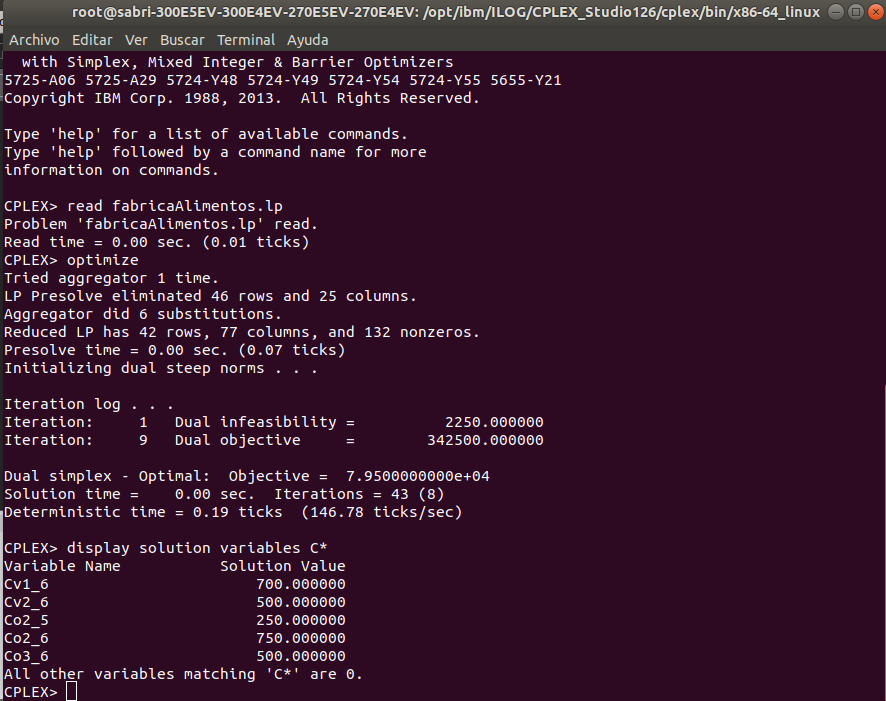
\includegraphics[scale=0.35]{modelos/fabricaAlimentos12-1Compras.png}
    \caption{Politicas de compras}
\end{figure}

\begin{figure}[!h]
    \centering
    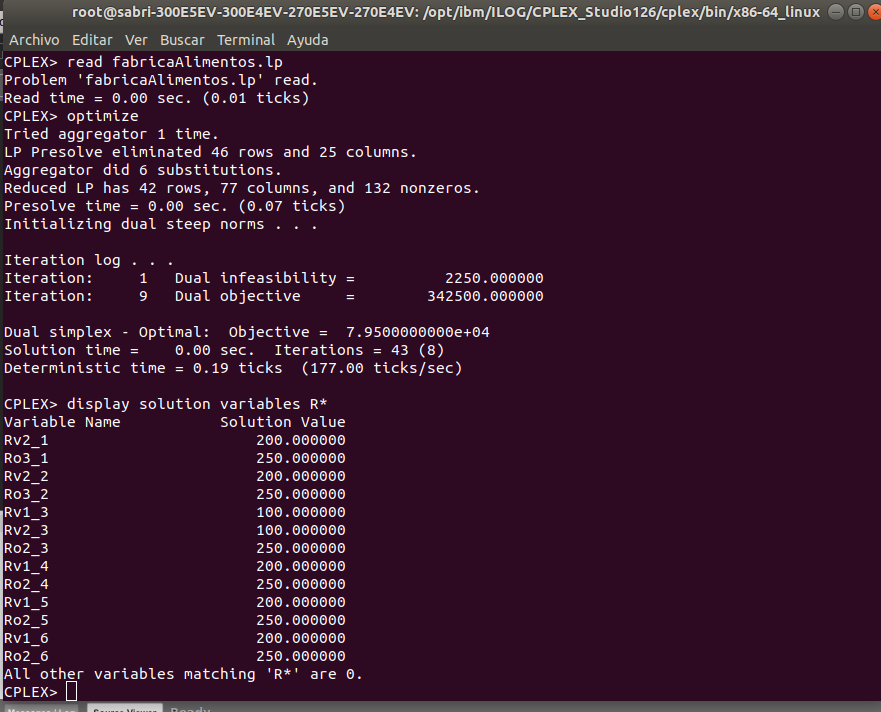
\includegraphics[scale=0.35]{modelos/fabricaAlimentos12-1Fabricacion.png}
    \caption{Politicas de fabricacion}
\end{figure}


\section{Fabricación de alimentos extensión}
\subsection{Enunciado 12-2}
\paragraph{}El problema y el problema posterior se basan en un modelo mas grande construido para el productor de margarina.
\paragraph{}Se desea imponer las siguientes condiciones adicionales al problema de la fabricación de alimentos.
\begin{itemize}
\item La comida nunca puede estar compuesta de mas de tres aceites en un mes.
\item Si se usa un aceite en un mes, se deben usar al menos 20 toneladas.
\item Si se utiliza Veg 1 o Veg 2 en un mes, también se deben utilizar oil 3.
\end{itemize}
\subsection{Modelo 12-2}
$\begin{array}{l}
Xv_{i,j} = \left\{
\begin{array}{l l}
 1 & \mbox{si } Rv_{i,j}>0\\
 0 & sino
\end{array}
\right.\\
Xo_{t,j} = \left\{
\begin{array}{l l}
 1 & \mbox{si } Ro_{i,j}>0\\
 0 & sino
\end{array}
\right.
\end{array}$
\\ \\ 
s.a\\
\begin{equation}
Xv_{1,j} + Xv_{2,j} + Xo_{1,j} + Xo_{2,j} + Xo_{3,j} \leq 3
\end{equation}
\begin{equation}
Rv_{i,j} \geq 20 \times Xv_{i,j}
\end{equation}
\begin{equation}
Ro_{t,j} \geq 20 \times Xo_{t,j}
\end{equation}
\begin{equation}
Rv_{1,j} \leq Ro_{3,j}
\end{equation}
\begin{equation}
Rv_{2,j} \leq Ro_{3,j}
\end{equation}

    \newpage
    \subsection{Optimización de refinería}
\subsubsection{Enunciado}
\paragraph{} Una refinería de aceite compra dos aceites crudos (crudo 1 y crudo 2). Estos aceites crudos se someten a cuatro procesos: destilación, reforma, craqueo y mezclado, para producir gasolinas y combustibles que se venden.
\paragraph{Distilación} La destilación separa cada aceite crudo en fracciones conocidas como nafta liviana, nafta media, nafta pesada, aceite liviano, aceite pesado y residuos según sus puntos de ebullición. Las naftas ligeras, medianas y pesadas tienen números de octano de 90, 80 y 70, respectivamente. Cada barril crudo produce: \\
\begin{center}
\begin{tabular}{ccccccc}
\hline 
 & Nafta & Nafta & Nafta & Aceite & Aceite & Residuos \\ 
 & liviana & media & pesada & liviano & pesado &  \\ 
\hline 
Crudo 1 & 0.1 & 0.2 & 0.2 & 0.12 & 0.2 & 0.13 \\ 
Crudo 2 & 0.15 & 0.25 & 0.18 & 0.08 & 0.19 & 0.12 \\ 
\hline 
\end{tabular} 
\end{center}
\paragraph{Reforma} Las naftas pueden usarse inmediatamente para mezclarse en diferentes grados de gasolina o pueden pasar por un proceso conocido como reforma. La reforma produce un producto conocido como gasolina reformada con un índice de octano de 115. Los rendimientos de gasolina reformada de cada barril de las diferentes naftas se dan de la siguiente manera:
\begin{itemize}
\item El barril de nafta liviana produce 0.6 barriles de gasolina reformada.
\item El barril de nafta mediana produce 0.52 barriles de gasolina reformada.
\item El barril de nafta pesada produce 0.45 barriles de gasolina reformada.
\end{itemize} 
\paragraph{Craqueo} 
Los aceites (livianos y pesados) se pueden usar directamente para mezclarlos en combustible para aviones o aceite combustible mediante un proceso conocido como craqueo catalítico. El craqueador catalítico produce aceite craqueado y gasolina craqueada. La gasolina craqueada tiene un octanaje de 105. 
\begin{itemize}
\item El barril de aceite liviano produce 0,68 barriles de aceite craqueado y 0,28 barriles de gasolina craqueada;
\item El barril de aceite pesado produce 0,75 barriles de aceite craqueado y 0,20 barriles de gasolina craqueada
\end{itemize} 
\paragraph{} El aceite craqueado se usa para mezclar aceite combustible y combustible para aviones; gasolina craqueada se utiliza para mezclar gasolina.
\paragraph{} Residuo se puede usar para producir aceite lubricante o mezclarlo en combustible para aviones y aceite combustible:
\begin{itemize}
\item El barril de residuos produce 0.5 barriles de aceite lubricante.
\end{itemize} 
\paragraph{Mezcla}
\begin{description}
\item[Gasolinas(combustible de motor)] Hay dos tipos de gasolina, regular y premium, obtenidos mezclando la nafta, la gasolina reformada y la gasolina crakeada. Las únicas restricciones que deben cumplir es que la gasolina regular debe tener un octanaje de al menos 84 y la premium al menos 94. Se supone que los números de octano se mezclan linealmente por volumen.
\item[Combustible para aviones] La restricción con respecto al combustible para aviones es que su presión de vapor no debe exceder 1 kg cm2. Las presiones de vapor para aceites ligeros, pesados, craquedos y residuos son 1.0, 0.6, 1.5 y 0.05 kg cm2, respectivamente. Se puede suponer nuevamente que las presiones de vapor se mezclan linealmente por volumen.
\item[Aceite combustible] Para producir aceite combustible, aceite craqueado, aceite liviano, aceite pesado y residuo se deben mezclar en una proporción de 10: 4: 3: 1.\\
Existen limitaciones de disponibilidad y capacidad en las cantidades y procesos utilizados de la siguiente manera:
\begin{enumerate}
\item La disponibilidad diaria de crudo 1 es de 20000 barriles.
\item La disponibilidad diaria de crudo 2 es de 30000 barriles.
\item Como máximo 45000 barriles de crudo se pueden destilar por día.
\item Como máximo se pueden reformar 10000 barriles de nafta por día.
\item Como máximo 8000 barriles de aceite pueden ser craqueados por día.
\item La producción diaria de aceite lubricante debe estar entre 500 y 1000 barriles.
\item La gasolina premium debe ser al menos el 40\% de la producción de la gasolina regular.
\end{enumerate}
Las contribuciones de ganancias de la venta de los productos finales son (en peniques por barril) de la siguiente manera:\\
\begin{center}
\begin{tabular}{cc}
\hline 
Gasolina premium & 700 \\ 
Gasolina regular & 600 \\ 
Combustible para aviones & 400 \\ 
Aceite combustible & 350 \\ 
Aceite lubricante & 150 \\ 
\hline 
\end{tabular} 
\end{center}
\end{description}
\paragraph{}¿Cómo deberían planificarse las operaciones de la refinería para maximizar el beneficio total?
\subsubsection{Modelo}

$\begin{array}{l}
C_{i}:\mbox{cantidad de barriles de crudo i}\\
D_{i}:\mbox{cantidad destilado de barriles de crudo i}\\
NL:\mbox{cantidad de nafta liviana obtenida en el proceso de destilacion}\\
NM:\mbox{cantidad de nafta mediana obtenida en el proceso de destilacion}\\
NP:\mbox{cantidad de nafta pesada obtenida en el proceso de destilacion}\\
NL_{t}:\mbox{cantidad de nafta liviana usada para mezclar gasolina en t}\\
NM_{t}:\mbox{cantidad de nafta mediana usada para mezclar gasolina en t}\\
NP_{t}:\mbox{cantidad de nafta pesada usada para mezclar gasolina en t}\\
NLR:\mbox{cantidad de nafta liviana que se puede refinar}\\
NMR:\mbox{cantidad de nafta mediana que se puede refinar}\\
NPR:\mbox{cantidad de nafta pesada que se puede refinar}\\
GR_{t}:\mbox{cantidad de gasolina reformada usada para mezclar gasolina en t}\\
AL:\mbox{cantidad de aceite liviano obtenida en el proceso de destilacion}\\
AP:\mbox{cantidad de aceite pesado obtenida en el proceso de destilacion}\\
AL_{s}:\mbox{cantidad de aceite liviano usado para mezclar en s}\\
AP_{s}:\mbox{cantidad de aceite pesado usado para mezclar en s}\\
ALC:\mbox{cantidad de aceite liviano que se puede craquear}\\
APC:\mbox{cantidad de aceite pesado que se puede craquear}\\
GC_{t}:\mbox{cantidad de gasolina crakeada usada para mezclar gasolina en t}\\
AC_{s}:\mbox{cantidad de aceite crakeado para mezclar en s}\\

R_{q}:\mbox{cantidad de residuo para mezclar en q}\\
GPrem:\mbox{cantidad gasolina premiun mezclada}\\
GRegu:\mbox{cantidad gasolina regular mezclada}\\
CAvion:\mbox{cantidad combustible de avion mezclado}\\
AComb:\mbox{cantidad aceite combustible mezclado}\\
ALu:\mbox{cantidad de aceite lubricante}\\
\mbox{donde} \;\;\;\;\;\; i=1,2 \;\;\;\;\;\; t=p,r  \;\;\;\;\;\; s=ca,ac \;\;\;\;\;\; q=ca,ac,al  
\end{array}$

$$ \mbox{max } 700 \mbox{ GPrem} + 600 \mbox{ GRegu} + 400 \mbox{ CAvion} + 350 \mbox{ AComb} + 150 \mbox{ ALu} $$
\\ \\
\\ \\ 
s.a\\
\begin{equation}
C_{1} \leq 20000 
\end{equation}
\begin{equation}
C_{2} \leq 30000 
\end{equation}
\begin{equation}
D_{1} \leq C_{1} 
\end{equation}
\begin{equation}
D_{2} \leq C_{2} 
\end{equation}
\begin{equation}
D_{1} + D_{2} \leq 45000 
\end{equation}
%como maximo se pueden reformar 1000 barriles de nafta por dia: nafta liviana: 0.1C_{1}+0.15C_{2}, nafta mediana  0.2C_{1}+0.25C_{2}, nafta pesada  0.2C_{1}+0.18C_{2}
\begin{equation}
NL = 0.1D_{1}+0.15D_{2} 
\end{equation}
\begin{equation}
NM = 0.2D_{1}+0.25D_{2} 
\end{equation}
\begin{equation}
NP = 0.2D_{1}+0.18D_{2} 
\end{equation}
\begin{equation}
NL_{p} + NL_{r} \leq NL 
\end{equation}
\begin{equation}
NM_{p} + NM_{r} \leq NM 
\end{equation}
\begin{equation}
NP_{p} + NP_{r} \leq NP 
\end{equation}
\begin{equation}
NLR = NL - (NL_{p} + NL_{r}) 
\end{equation}
\begin{equation}
NMR = NM - (NM_{p} + NM_{r}) 
\end{equation}
\begin{equation}
NPR = NP - (NP_{p} + NP_{r}) 
\end{equation}
\begin{equation}
GR_{p} + GR_{r} \leq 0.6 NLR + 0.52 NMR + 0.45 NPR 
\end{equation}
\begin{equation}
NLR + NMR + NPR \leq 10000 
\end{equation}
\begin{equation}
AL = 0.12D_{1}+0.08D_{2}
\end{equation}
\begin{equation}
AP = 0.19D_{1}+0.12D_{2}
\end{equation}
\begin{equation}
AL_{ca} + AL_{ac} \leq AL
\end{equation}
\begin{equation}
AP_{ca} + AP_{ac} \leq AP
\end{equation}
\begin{equation}
ALC = AL - (AL_{ca} + AL_{ac})
\end{equation}
\begin{equation}
APC = AP - (AP_{ca} + AP_{ac})
\end{equation}
\begin{equation}
ALC + APC \leq 8000 
\end{equation}
\begin{equation}
AC_{ca} + AC_{ac} \leq 0.68 ALC + 0.75 APC
\end{equation}
\begin{equation}
GC_{p} + GC_{r} \leq 0.28 ALC + 0.20 APC
\end{equation}
\begin{equation}
R_{ca} + R_{ac} + R_{al} \leq 0.13D_{1} + 0.12D_{2} 
\end{equation}
\begin{equation}
ALu \leq 0.5 R_{al} 
\end{equation}
\begin{equation}
ALu \geq 500 
\end{equation}
\begin{equation}
ALu \leq 1000 
\end{equation}
\begin{equation}
GPrem \leq NL_{p}+NM_{p}+NP_{p}+GR_{p}+GC_{p}
\end{equation}
\begin{equation}
GReg \leq NL_{r}+NM_{r}+NP_{r}+GR_{r}+GC_{r}
\end{equation}
\begin{equation}
(90NL_{p}+80NM_{p}+70NP_{p}+115GR_{p}+105GC_{p}) \div GPrem \geq 94 
\end{equation}
\begin{equation}
(90NL_{r}+80NM_{r}+70NP_{r}+115GR_{r}+105GC_{r}) \div GReg \geq 84 
\end{equation}
\begin{equation}
(GPrem \times 100) \div GReg \leq 40 
\end{equation}
\begin{equation}
CAvion \leq AL_{ca}+AP_{ca}+ AC_{ca}+ R_{ca}
\end{equation}
\begin{equation}
(1.0AL_{ca}+0.6AP_{ca}+1.5AC_{ca}+0.05R_{ca}) \div CAvion \leq 1 
\end{equation}
\begin{equation}
AComb \leq (1/10)AL_{ac}+(1/4)AP_{ac}+ (1/3)AC_{ac}+ R_{ac}
\end{equation}

\subsubsection{Modelo CPLEX}
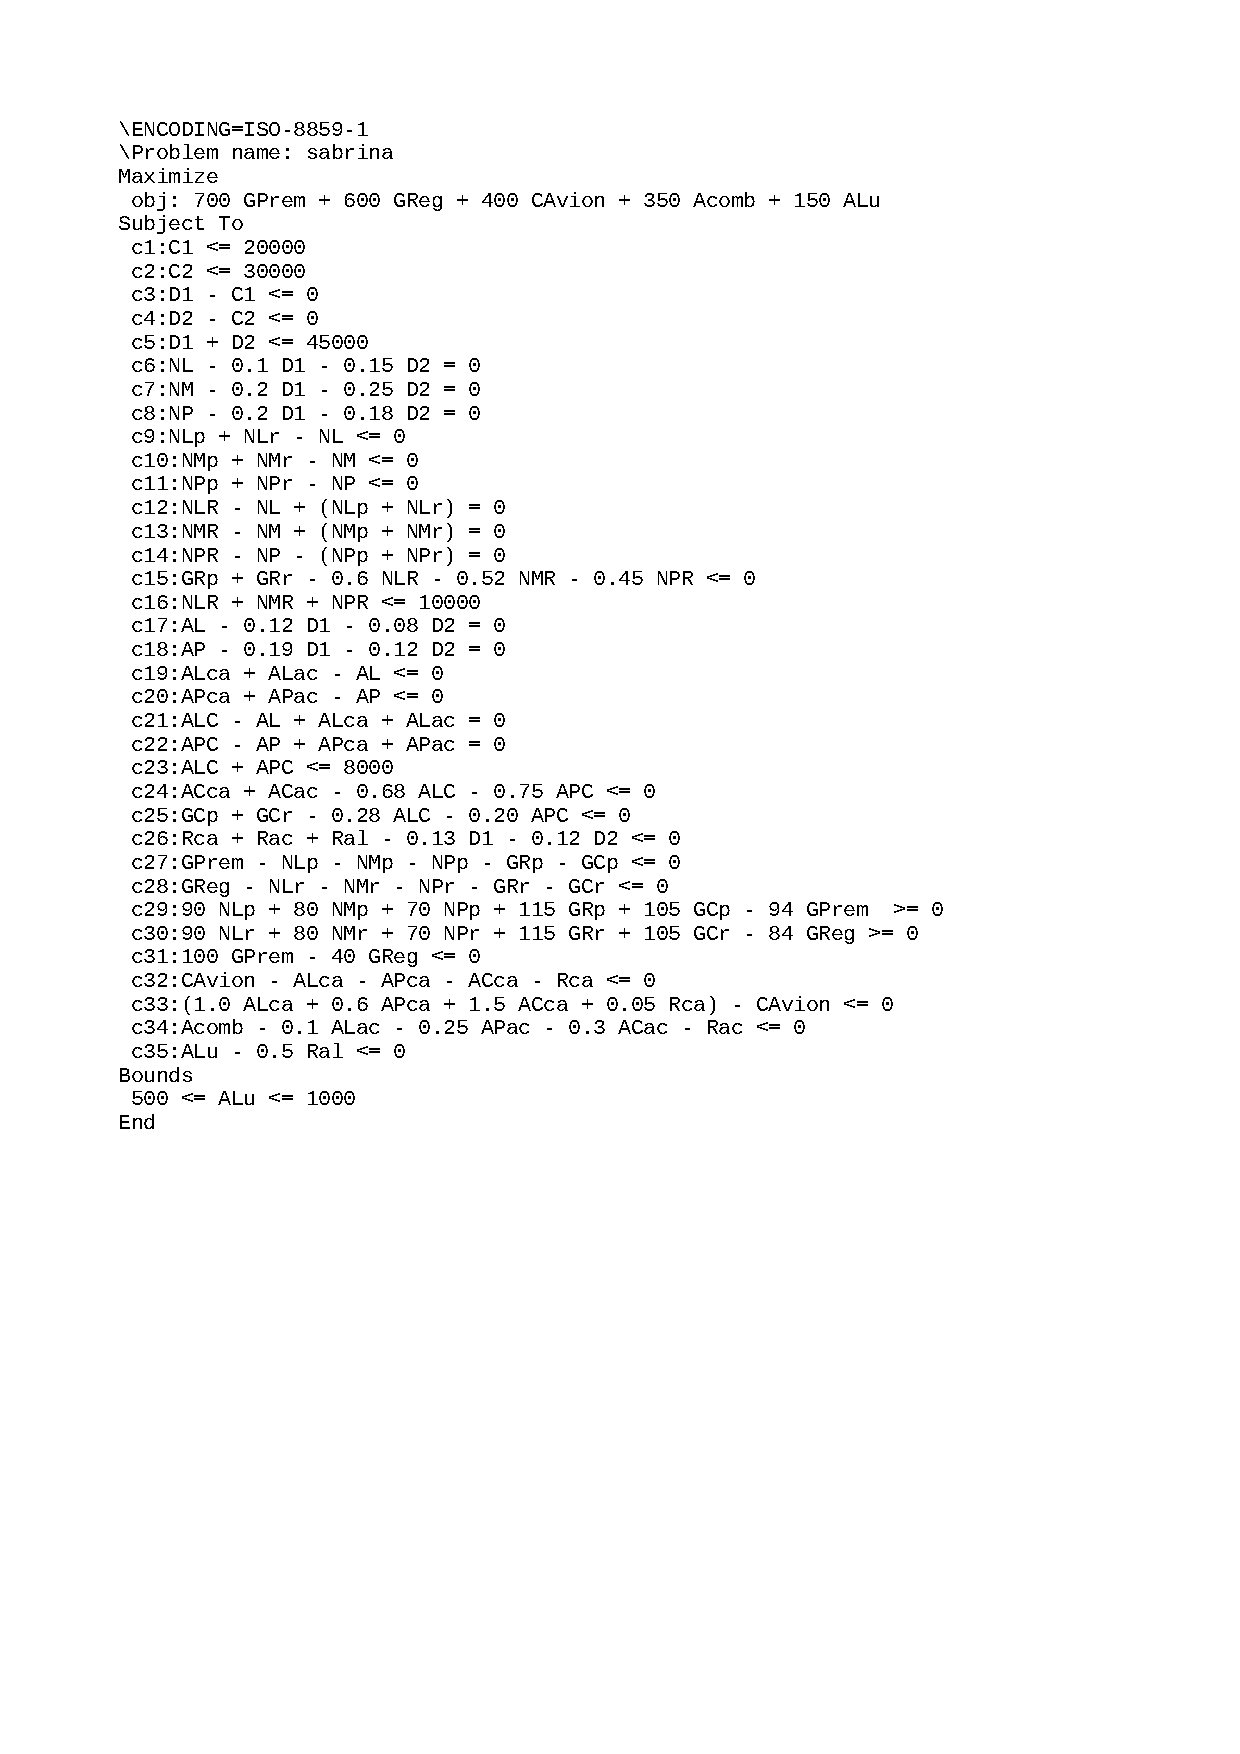
\includepdf[pages=1]{modelos/refineria}
\subsubsection{Solucion CPLEX}
\begin{figure}[!h]
    \centering
    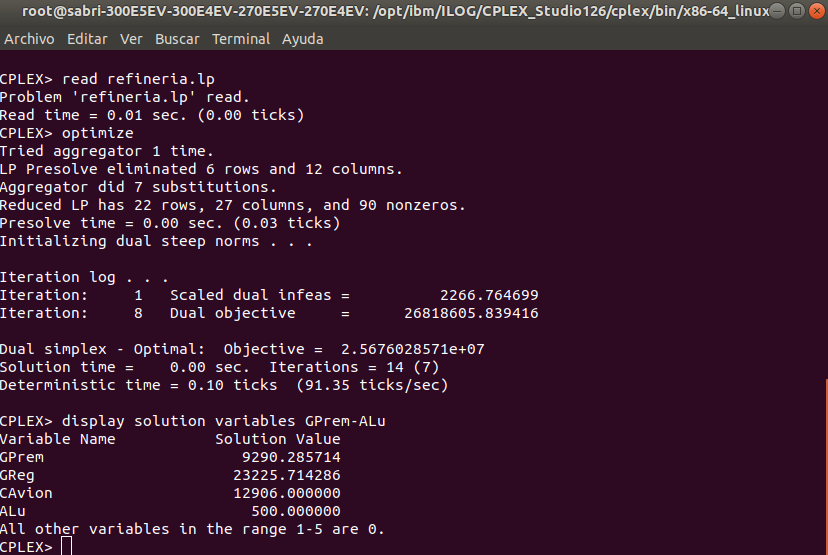
\includegraphics[scale=0.4]{modelos/SolutionRefineria.png}
    \caption{SolucionRefineria}
\end{figure}


    \newpage
    \section{Mercado compartido}
\subsection{Enunciado}
\paragraph{} Una compañía grande tiene dos divisiones, D1 y D2. La compañía provee a los minoristas con aceite y alcohol. Esta es una versión mucho más pequeña del problema al que se enfrentaron British Petroleum y Shell cuando se vieron obligados a abandonar, una de las divisiones más grandes de la historia. El modelo original resultó imposible de resolver en 1972.
\paragraph{} Se desea asignar a cada minorista una división D1 o D2. Esta división será el proveedor del minorista. En la medida de lo posible, esta división debe realizarse de modo que D1 controle el 40\% del mercado y D2 el 60\% restante. Los minoristas se enumeran a continuación como M1 a M23. Cada minorista tiene un mercado estimado para aceite y alcohol. Los minoristas M1 a M8 están en la región 1; los minoristas M9 a M18 están en la región 2 y los minoristas M19 a M23 están en la región 3. Se considera que algunos minoristas tienen buenas perspectivas de crecimiento y se clasifican en el grupo A y los otros en el grupo B. Cada minorista tiene un cierto número de puntos de entrega, como se indica a continuación. Se desea dividir la división 40/60 entre D1 y D2 en cada uno de los siguientes aspectos:
\begin{enumerate}
\item Número total de puntos de entrega
\item Control de mercado de alcohol
\item Control de mercado de aceite en la región 1
\item Control de mercado de aceite en la región 2
\item Control de mercado de aceite en la región 3
\item Numero de minoristas en el grupo A
\item Numero de minoristas en el grupo B
\end{enumerate}
\paragraph{} Existe cierta flexibilidad en cuanto a que cualquier acción puede variar en $\pm$ 5\%. Esa es la parte puede muy entre los límites 35/65 y 45/55.
\paragraph{} El objetivo principal es encontrar una solución factible. Sin embargo, si hay alguna opción, los posibles objetivos son (i) minimizar la suma de las desviaciones porcentuales de la división 40/60 y (ii) minimizar la desviación máxima.
\paragraph{} Cree un modelo para ver si el problema tiene una solución viable y, de ser así, encuentre las soluciones óptimas.
\paragraph{} Los datos numéricos se dan en la siguiente tabla:

\subsection{Modelo}
$\begin{array}{l}
D1PEM_{i}:\mbox{indica si M i esta en la división D1 segun el punto de entrega}\\
TD1PE:\mbox{total de puntos de entrega de los M i en la división D1}\\
PorcPuntoEntregaD1:\mbox{pocentaje de puntos de entrega de los M i en la división D1}\\
D2PEaM_{i}:\mbox{indica si M i esta en la división D2 segun el punto de entrega}\\
TD2PE:\mbox{total de puntos de entrega de los M i en la división D2}\\
PorcPuntoEntregaD2:\mbox{pocentaje de puntos de entrega de los M i en la división D2}\\
D1MAM_{i}:\mbox{indica si M i esta en la división D1 segun el mercado de alcohol}\\
TD1MA:\mbox{total de mercado alcohol de los M i en la división D1}\\
PorcMAlcoholD1:\mbox{porcentaje de mercado alcohol de los M i en la división D1}\\
D2MAM_{i}:\mbox{indica si M i esta en la división D2 segun el mercado de alcohol}\\
TD2MA:\mbox{total de mercado alcohol de los M i en la división D2}\\
PorcMAlcoholD2:\mbox{porcentaje de mercado alcohol de los M i en la división D2}\\
D1R1M_{i}:\mbox{indica si M i esta en la división D1 segun la región 1}\\
TD1R1:\mbox{total de region 1 de los M i en la división D1}\\
PorcRegion1D1:\mbox{porcentaje de region 1 de los M i en la división D1}\\
D2R1M_{i}:\mbox{indica si M i esta en la división D2 segun la región 1}\\
TD2R1:\mbox{total de region 1 de los M i en la división D2}\\
PorcRegion1D2:\mbox{porcentaje de region 1 de los M i en la división D2}\\
D1R2M_{i}:\mbox{indica si M i esta en la división D1 segun la región 2}\\
TD1R2:\mbox{total de region 2 de los M i en la división D1}\\
PorcRegion2D1:\mbox{porcentaje de region 2 de los M i en la división D1}\\
D2R2M_{i}:\mbox{indica si M i esta en la división D2 segun la región 2}\\
TD2R2:\mbox{total de region 2 de los M i en la división D2}\\
PorcRegion2D2:\mbox{porcentaje de region 2 de los M i en la división D2}\\
D1R3M_{i}:\mbox{indica si M i esta en la división D1 segun la región 3}\\
TD1R3:\mbox{total de region 3 de los M i en la división D1}\\
PorcRegion3D1:\mbox{porcentaje de region 3 de los M i en la división D1}\\
D2R3M_{i}:\mbox{indica si M i esta en la división D2 segun la región 3}\\
TD2R3:\mbox{total de region 3 de los M i en la división D2}\\
PorcRegion3D2:\mbox{porcentaje de region 3 de los M i en la división D2}\\
D1GAM_{i}:\mbox{indica si M i esta en la división D1 segun grupo A}\\
TD1GA:\mbox{total de categoria A de los M i en la división D1}\\
PorcGrupoAD1:\mbox{porcentaje de categoria A de los M i en la división D1}\\
D2GAM_{i}:\mbox{indica si M i esta en la división D2 segun grupo A}\\
TD2GA:\mbox{total de categoria A de los M i en la división D2}\\
PorcGrupoAD2:\mbox{porcentaje de categoria A de los M i en la división D2}\\
D1GBM_{i}:\mbox{indica si M i esta en la división D1 segun grupo B}\\
TD1GB:\mbox{total de categoria B de los M i en la división D1}\\
PorcGrupoBD1:\mbox{porcentaje de categoria B de los M i en la división D1}\\
D2GBM_{i}:\mbox{indica si M i esta en la división D2 segun grupo B}\\
TD2GB:\mbox{total de categoria B de los M i en la división D2}\\
PorcGrupoBD2:\mbox{porcentaje de categoria B de los M i en la división D2}\\
%\mbox{donde} \;\;\;\;\;\; i=1,2,3, \ldots , 23  
\end{array}$
\\ \\
$$ \mbox{max } $$
\\ 
sujeto a\\\\
Suma total de puntos de entrega de los minoristas M i en  D1 
\begin{equation*}
\begin{split}
  TD1PE = & 11 D1PEM_1 + 47 D1PEM_2 + 44 D1PEM_3 + 25 D1PEM_4 + \\ 
  		  & 10 D1PEM_5 + 26 D1PEM_6 + 26 D1PEM_7 + 54 D1PEM_8 + \\
  		  & 18 D1PEM_9 + 51 D1PEM_{10} + 20 D1PEM_{11} + 105 D1PEM_{12} + \\ 
  		  &  7 D1PEM_{13} + 16 D1PEM_{14} + 34 D1PEM_{15} + 100 D1PEM_{16} + \\ 
  		  & 50 D1PEM_{17} + 21 D1PEM_{18} + 11 D1PEM_{19} + 19 D1PEM_{20} + \\
		  & 14 D1PEM_{21} + 10 D1PEM_{22} + 11 D1PEM_{23} 
\end{split}
\end{equation*}
Suma total de puntos de entrega de los minoristas M i en  D2 
\begin{equation*}
\begin{split}
  TD2PE = & 11 D2PEM_1 + 47 D2PEM_2 + 44 D2PEM_3 + 25 D2PEM_4 + \\ 
  		  & 10 D2PEM_5 + 26 D2PEM_6 + 26 D2PEM_7 + 54 D2PEM_8 + \\
  		  & 18 D2PEM_9 + 51 D2PEM_{10} + 20 D2PEM_{11} + 105 D2PEM_{12} + \\ 
  		  &  7 D2PEM_{13} + 16 D2PEM_{14} + 34 D2PEM_{15} + 100 D2PEM_{16} + \\ 
  		  & 50 D2PEM_{17} + 21 D2PEM_{18} + 11 D2PEM_{19} + 19 D2PEM_{20} + \\
		  & 14 D2PEM_{21} + 10 D2PEM_{22} + 11 D2PEM_{23} 
\end{split}
\end{equation*}
La suma de los minorista de puntos de entrega en D1 y D2 deben ser 23
\begin{equation*}
\begin{split}
23 = & D1PEM_1 + D1PEM_2 + D1PEM_3 + D1PEM_4 + D1PEM_5 + D1PEM_6 + \\
     & D1PEM_7 + D1PEM_8 + D1PEM_9 + D1PEM_{10} + D1PEM_{11} + D1PEM_{12} +\\
     & D1PEM_{13} + D1PEM_{14} + D1PEM_{15} + D1PEM_{16} + D1PEM_{17} + \\
     & D1PEM_{18} + D1PEM_{19} + D1PEM_{20} + D1PEM_{21} + D1PEM_{22} + \\
	 & D1PEM_{23} + D2PEM_1 + D2PEM_2 + D2PEM_3 + D2PEM_4 + D2PEM_5 + \\
	 & D2PEM_6 + D2PEM_7 + D2PEM_8 + D2PEM_9 + D2PEM_{10} + D2PEM_{11} + \\
	 & D2PEM_{12} + D2PEM_{13} + D2PEM_{14} + D2PEM_{15} + D2PEM_{16} + D2PEM_{17} +\\
	 & D2PEM_{18} + D2PEM_{19} + D2PEM_{20} + D2PEM_{21} + D2PEM_{22} + D2PEM_{23}
\end{split}
\end{equation*}
Suma total de mercado alcohol de los M i en la división D1
\begin{equation*}
\begin{split}
  TD1MA = & 34  D1MAM_1 + 411 D1MAM_2 + 82 D1MAM_3 + 157 D1MAM_4 + \\ 
  		  &  5  D1MAM_5 + 183 D1MAM_6 + 14 D1MAM_7 + 215 D1MAM_8 + \\
  		  & 102 D1MAM_9 + 21  D1MAM_{10} + 54 D1MAM_{11} + 0 D1MAM_{12} + \\ 
  		  &  6 D1MAM_{13} + 96 D1MAM_{14} + 118 D1MAM_{15} + 112 D1MAM_{16} + \\ 
  		  & 535 D1MAM_{17} + 8 D1MAM_{18} +  53 D1MAM_{19} + 28 D1MAM_{20} + \\
		  & 69 D1MAM_{21} + 65 D1MAM_{22} + 27 D1MAM_{23} 
\end{split}
\end{equation*}
Suma total de mercado alcohol de los M i en la división D2
\begin{equation*}
\begin{split}
  TD2MA = & 34 D2MAM_1 + 411 D2MAM_2 + 82 D2MAM_3 + 157 D2MAM_4 + \\ 
  		  & 5 D2MAM_5 + 183 D2MAM_6 + 14 D2MAM_7 + 215 D2MAM_8 + \\
  		  & 102 D2MAM_9 + 21 D2MAM_{10} + 54 D2MAM_{11} + 0 D2MAM_{12} + \\ 
  		  & 6 D2MAM_{13} + 96 D2MAM_{14} + 118 D2MAM_{15} + 112 D2MAM_{16} + \\ 
  		  & 535 D2MAM_{17} + 8 D2MAM_{18} +  53 D2MAM_{19} + 28 D2MAM_{20} + \\
		  & 69 D2MAM_{21} + 65 D2MAM_{22} + 27 D2MAM_{23} 
\end{split}
\end{equation*}

La suma de los minorista de mercado alcohol en D1 y D2 deben ser 23
\begin{equation*}
\begin{split}
23 =  	&  D1MAM_1 + D1MAM_2 + D1MAM_3 + D1MAM_4 + D1MAM_5 +\\ 
      	&  D1MAM_6 + D1MAM_7 + D1MAM_8 + D1MAM_9 + D1MAM_{10} +\\
  		&  D1MAM_{11} + D1MAM_{12} + D1MAM_{13} + D1MAM_{14} +\\ 
  		&  D1MAM_{15} + D1MAM_{16} + D1MAM_{17} + D1MAM_{18} + \\ 
  		&  D1MAM_{19} + D1MAM_{20} + D1MAM_{21} + D1MAM_{22} + \\
		&  D1MAM_{23} + D2MAM_1 + D2MAM_2 + D2MAM_3 + D2MAM_4 +\\
		&  D2MAM_5 + D2MAM_6 + D2MAM_7 + D2MAM_8 + D2MAM_9 + \\
		&  D2MAM_{10} + D2MAM_{11} + D2MAM_{12} +  D2MAM_{13} + \\
		&  D2MAM_{14} + D2MAM_{15} + D2MAM_{16} + D2MAM_{17} + \\
		&  D2MAM_{18} + D2MAM_{19} + D2MAM_{20} + D2MAM_{21} + \\
		&  D2MAM_{22} + D2MAM_{23}\\
\end{split}
\end{equation*}



Total mercado aceite region 1 de los M i en la división D1
\begin{equation*}
\begin{split}
  TD1R1 = &  9 D1R1M_1 + 13 D1R1M_2 + 14 D1R1M_3 + 17 D1R1M_4 + \\ 
  		  & 18 D1R1M_5 + 19 D1R1M_6 + 23 D1R1M_7 + 21 D1R1M_8
\end{split}
\end{equation*}
Total mercado aceite region 1 de los M i en la división D2
\begin{equation*}
\begin{split}
  TD2R1 = &  9 D2R1M_1 + 13 D2R1M_2 + 14 D2R1M_3 + 17 D2R1M_4 + \\ 
  		  & 18 D2R1M_5 + 19 D2R1M_6 + 23 D2R1M_7 + 21 D2R1M_8 
\end{split}
\end{equation*}
Total mercado de aceite region 2 de los M i en la división D1
\begin{equation*}
\begin{split}
  TD1R2 = &  9 D1R2M_9 + 11 D1R2M_{10} + 17 D1R2M_{11} + 18 D1R2M_{12} + 18 D1R2M_{13} +\\ 
  		  & 17 D1R2M_{14} + 22 D1R2M_{15} + 24 D1R2M_{16} + 36 D1R2M_{17} + 43 D1R2M_{18}
\end{split}
\end{equation*}
Total mercado de aceite region 2 de los M i en la división D2
\begin{equation*}
\begin{split}
  TD2R2 = &  9 D2R2M_9 + 11 D2R2M_{10} + 17 D2R2M_{11} + 18 D2R2M_{12} + 18 D2R2M_{13} +\\ 
  		  & 17 D2R2M_{14} + 22 D2R2M_{15} + 24  D2R2M_{16} + 36 D2R2M_{17} + 43 D2R2M_{18}
\end{split}
\end{equation*}
Total mercado de aceite region 3 de los M i en la división D1
\begin{equation*}
\begin{split}
  TD1R3 = & 6 D1R3M_{19} + 15 D1R3M_{20} + 15 D1R3M_{21} + 25 D1R3M_{22} + 39 D1R3M_{23} 
\end{split}
\end{equation*}
Total mercado de aceite region 3 de los M i en la división D2
\begin{equation*}
\begin{split}
  TD2R3 = & 6 D2R3M_{19} + 15 D2R3M_{20} + 15 D2R3M_{21} + 25 D2R3M_{22} + 39 D2R3M_{23} 
\end{split}
\end{equation*}
La suma de los minorista de mercado de aceite de las regiones 1,2 y 3 de los M i en la división en D1 y D2 deben ser 23
\begin{equation*}
\begin{split}
23 =  	&  D1R1M_1 + D1R1M_2 + D1R1M_3 + D1R1M_4 + D1R1M_5 + D1R1M_6 + D1R1M_7 + D1R1M_8 \\
		& + D2R1M_1 + D2R1M_2 + D2R1M_3 + D2R1M_4 + D2R1M_5 + D2R1M_6 + D2R1M_7 + D2R1M_8 \\
		& + D1R2M_9 + D1R2M_{10} + D1R2M_{11} + D1R2M_{12} + D1R2M_{13} + D1R2M_{14} + D1R2M_{15} \\ 
		& + D1R2M_{16} + D1R2M_{17} + D1R2M_{18} + D2R2M_9 + D2R2M_{10} + D2R2M_{11} + D2R2M_{12} \\
		& + D2R2M_{13} + D2R2M_{14} + D2R2M_{15} + D2R2M_{16} + D2R2M_{17} + D2R2M_{18} + D1R3M_{19} \\
		& + D1R3M_{20} + D1R3M_{21} + D1R3M_{22} + D1R3M_{23} + D2R3M_{19} + D2R3M_{20} + D2R3M_{21} \\
		& + D2R3M_{22} + D2R3M_{23}
\end{split}
\end{equation*}
Total de categoria A de los M i en la división D1
\begin{equation*}
\begin{split}
  TD1GA = & D1GAM_1 + D1GAM_2 + D1GAM_3 + D1GAM_5 + D1GAM_6 +\\
          & D1GAM_{10} + D1GAM_{15} + D1GAM_{20} 
\end{split}
\end{equation*}
Total de categoria A de los M i en la división D2
\begin{equation*}
\begin{split}
  TD2GA = & D2GAM_1 + D2GAM_2 + D2GAM_3 + D2GAM_5 + D2GAM_6 +\\
          & D2GAM_{10} + D2GAM_{15} + D2GAM_{20} 
\end{split}
\end{equation*}
Total de categoria B de los M i en la división D1
\begin{equation*}
\begin{split}
  TD1GB = & D1GAM_4 + D1GAM_7 + D1GAM_8 + D1GAM_9 + D1GAM_{11} + \\
          & D1GAM_{12} + D1GAM_{13} + D1GAM_{14} + D1GAM_{16} + D1GAM_{17} +\\
          & D1GAM_{18} + D1GAM_{19} + D1GAM_{21} + D1GAM_{22} + D1GAM_{23}
\end{split}
\end{equation*}
Total de categoria B de los M i en la división D2
\begin{equation*}
\begin{split}
  TD2GB = & D2GAM_4 + D2GAM_7 + D2GAM_8 + D2GAM_9 + D2GAM_{11} +\\
          & D2GAM_{12} + D2GAM_{13} + D2GAM_{14} + D2GAM_{16} + D2GAM_{17} +\\
          & D2GAM_{18} + D2GAM_{19} + D2GAM_{21} + D2GAM_{22} + D2GAM_{23}
\end{split}
\end{equation*}
La suma de los minorista de la categoria A y B en la división en D1 y D2 deben ser 23
\begin{equation*}
\begin{split}
23 =  	&   D1GAM_1 + D1GAM_2 + D1GAM_3 + D1GAM_5 + D1GAM_6 +  D1GAM_{10} \\
	    & + D1GAM_{15} + D1GAM_{20} + D2GAM_1 + D2GAM_2 + D2GAM_3 + D2GAM_5 \\
	    & + D2GAM_6 + D2GAM_{10} + D2GAM_{15} + D2GAM_{20} + D1GAM_4 \\
	    & + D1GAM_7 + D1GAM_8 + D1GAM_9 + D1GAM_{11} + D1GAM_{12} + D1GAM_{13} \\
	    & + D1GAM_{14} + D1GAM_{16} + D1GAM_{17} + D1GAM_{18} + D1GAM_{19} \\
	    & + D1GAM_{21} + D1GAM_{22} + D1GAM_{23} + D2GAM_4 + D2GAM_7 + D2GAM_8 \\
	    & + D2GAM_9 + D2GAM_{11} + D2GAM_{12} + D2GAM_{13} + D2GAM_{14} \\
	    & + D2GAM_{16} + D2GAM_{17} + D2GAM_{18} + D2GAM_{19} + D2GAM_{21} \\
	    & + D2GAM_{22} + D2GAM_{23}
\end{split}
\end{equation*}


\paragraph{} Se desea hacer la división 40/60 entre D1 y D2, flexibilidad en cuanto a que cualquier acción puede variar en $\pm$ 5 \%, osea los límites 35/65 y 45/55.\\ 
\paragraph{Puntos de entrega} Obtenemos los porcentajes de los puntos de entrega de D1 y D2.  
\begin{equation}
PorcPuntoEntregaD1 = TD1PE \times 100 \div (TD1PE + TD2PE)
\end{equation}
\begin{equation}
PorcPuntoEntregaD2 = TD2PE \times 100 \div (TD1PE + TD2PE)
\end{equation}
La suma de los porcentajes tiene que ser igual al 100\%
\begin{equation}
PorcPuntoEntregaD1 + PorcPuntoEntregaD2 = 100
\end{equation}
D1 tiene que moverse entre 35 y 45 \%
\begin{equation}
PorcPuntoEntregaD1 \geq 35
\end{equation}
\begin{equation}
PorcPuntoEntregaD1 \leq 45
\end{equation}
D2 tiene que moverse entre 55 y 65 \%
\begin{equation}
PorcPuntoEntregaD2 \geq 55
\end{equation}
\begin{equation}
PorcPuntoEntregaD2 \leq 65
\end{equation}
\paragraph{Mercado de alcohol} Obtenemos los porcentajes de los mercados de alcohol de D1 y D2.  
\begin{equation}
PorcMAlcoholD1 = TD1MA \times 100 \div (TD1MA + TD2MA)
\end{equation}
\begin{equation}
PorcMAlcoholD2 = TD2MA \times 100 \div (TD1MA + TD2MA)
\end{equation}
La suma de los porcentajes tiene que ser igual al 100\%
\begin{equation}
PorcMAlcoholD1 + PorcMAlcoholD2 = 100
\end{equation}
D1 tiene que moverse entre 35 y 45 \%
\begin{equation}
PorcMAlcoholD1 \geq 35
\end{equation}
\begin{equation}
PorcMAlcoholD1 \leq 45
\end{equation}
D2 tiene que moverse entre 55 y 65 \%
\begin{equation}
PorcMAlcoholD2 \geq 55
\end{equation}
\begin{equation}
PorcMAlcoholD2 \leq 65
\end{equation}
\paragraph{Región 1} Obtenemos los porcentajes de la región 1 de D1 y D2.  
\begin{equation}
PorcRegion1D1 = TD1R1 \times 100 \div (TD1R1 + TD2R1)
\end{equation}
\begin{equation}
PorcRegion1D2 = TD2R1 \times 100 \div (TD1R1 + TD2R1)
\end{equation}
La suma de los porcentajes tiene que ser igual al 100\%
\begin{equation}
PorcRegion1D1 + PorcRegion1D2 = 100
\end{equation}
D1 tiene que moverse entre 35 y 45 \%
\begin{equation}
PorcRegion1D1 \geq 35
\end{equation}
\begin{equation}
PorcRegion1D1 \leq 45
\end{equation}
D2 tiene que moverse entre 55 y 65 \%
\begin{equation}
PorcRegion1D2 \geq 55
\end{equation}
\begin{equation}
PorcRegion1D2 \leq 65
\end{equation}
\paragraph{Región 2} Obtenemos los porcentajes de la región 2 de D1 y D2.  
\begin{equation}
PorcRegion2D1 = TD1R2 \times 100 \div (TD1R2 + TD2R2)
\end{equation}
\begin{equation}
PorcRegion2D2 = TD2R2 \times 100 \div (TD1R2 + TD2R2)
\end{equation}
La suma de los porcentajes tiene que ser igual al 100\%
\begin{equation}
PorcRegion2D1 + PorcRegion2D2 = 100
\end{equation}
D1 tiene que moverse entre 35 y 45 \%
\begin{equation}
PorcRegion2D1 \geq 35
\end{equation}
\begin{equation}
PorcRegion2D1 \leq 45
\end{equation}
D2 tiene que moverse entre 55 y 65 \%
\begin{equation}
PorcRegion2D2 \geq 55
\end{equation}
\begin{equation}
PorcRegion2D2 \leq 65
\end{equation}
\paragraph{Región 3} Obtenemos los porcentajes de la región 3 de D1 y D2.  
\begin{equation}
PorcRegion3D1 = TD1R3 \times 100 \div (TD1R3 + TD2R3)
\end{equation}
\begin{equation}
PorcRegion3D2 = TD2R3 \times 100 \div (TD1R3 + TD2R3)
\end{equation}
La suma de los porcentajes tiene que ser igual al 100\%
\begin{equation}
PorcRegion3D1 + PorcRegion3D2 = 100
\end{equation}
D1 tiene que moverse entre 35 y 45 \%
\begin{equation}
PorcRegion3D1 \geq 35
\end{equation}
\begin{equation}
PorcRegion3D1 \leq 45
\end{equation}
D2 tiene que moverse entre 55 y 65 \%
\begin{equation}
PorcRegion3D2 \geq 55
\end{equation}
\begin{equation}
PorcRegion3D2 \leq 65
\end{equation}
\paragraph{Grupo A} Obtenemos los porcentajes del grupo A de D1 y D2.  
\begin{equation}
PorcGrupoAD1 = TD1GA \times 100 \div (TD1GA + TD2GA)
\end{equation}
\begin{equation}
PorcGrupoAD2 = TD2GA \times 100 \div (TD1GA + TD2GA)
\end{equation}
La suma de los porcentajes tiene que ser igual al 100\%
\begin{equation}
PorcGrupoAD1 + PorcGrupoAD2 = 100
\end{equation}
D1 tiene que moverse entre 35 y 45 \%
\begin{equation}
PorcGrupoAD1 \geq 35
\end{equation}
\begin{equation}
PorcGrupoAD1 \leq 45
\end{equation}
D2 tiene que moverse entre 55 y 65 \%
\begin{equation}
PorcGrupoAD2 \geq 55
\end{equation}
\begin{equation}
PorcGrupoAD2 \leq 65
\end{equation}
\paragraph{Grupo B} Obtenemos los porcentajes del grupo B de D1 y D2.  
\begin{equation}
PorcGrupoBD1 = TD1GB \times 100 \div (TD1GB + TD2GB)
\end{equation}
\begin{equation}
PorcGrupoBD2 = TD2GB \times 100 \div (TD1GB + TD2GB)
\end{equation}
La suma de los porcentajes tiene que ser igual al 100\%
\begin{equation}
PorcGrupoBD1 + PorcGrupoBD2 = 100
\end{equation}
D1 tiene que moverse entre 35 y 45 \%
\begin{equation}
PorcGrupoBD1 \geq 35
\end{equation}
\begin{equation}
PorcGrupoBD1 \leq 45
\end{equation}
D2 tiene que moverse entre 55 y 65 \%
\begin{equation}
PorcGrupoBD2 \geq 55
\end{equation}
\begin{equation}
PorcGrupoBD2 \leq 65
\end{equation}

    \newpage
    \section{Generación de energía}
\subsection{Enunciado 12.5}
\paragraph{} Varias centrales eléctricas se comprometen a cumplir las siguientes demandas de carga de electricidad durante un día:\\
\begin{center}
\begin{tabular}{cc}
\hline 
12 pm a 6 am & 15000 MW \\  
6 am a 9 am & 30000 MW \\  
9 am a 3 pm & 25000 MW \\  
3 pm a 6 pm & 40000 MW \\  
6 pm a 12 pm & 27000 MW \\ 
\hline 
\end{tabular} 
\end{center}

\paragraph{} Hay tres tipos de unidades generadoras disponibles: 12 de tipo 1, 10 de tipo 2 y cinco de tipo 3. Cada generador tiene que funcionar entre un nivel mínimo y un nivel máximo. Hay un costo por hora de funcionamiento de cada generador al nivel mínimo. Además, hay un costo adicional por hora por cada megavatio en el que se opera una unidad por encima del nivel mínimo. Iniciar un generador también implica un costo. Toda esta información se da en la tabla 12.6 (con costos en \pounds).
\begin{center}
\begin{tabular}{cccccc}
\hline 
 & Nivel & Nivel & Costo por  & Costo por hora & Costo \\ 
 & Minimo & Maximo & hora como & por megavatio &  \\ 
 &  &  & minimo & $>$ minimo &  \\ 
\hline 
Type 1 & 850 MW & 2000 MW & 1000 & 2 & 2000 \\ 
Type 2 & 1250 MW & 1750 MW & 2600 & 1.30 & 1000 \\ 
Type 3 & 1500 MW & 4000 MW & 3000 & 3 & 500 \\ 
\hline 
\end{tabular} 
\end{center}

\paragraph{} Además de cumplir con las demandas de carga estimadas, debe haber suficientes generadores trabajando en todo momento para que sea posible cumplir con un aumento en la carga de hasta 15\%. Este aumento tendría que lograrse ajustando la producción de los generadores que ya operan dentro de sus límites permitidos.

\paragraph{} ¿Qué generadores deberían estar trabajando en qué períodos del día para minimizar el costo total?

\paragraph{} ¿Cuál es el costo marginal de producción de electricidad en cada período del día?; es decir, ¿qué aranceles deberían cobrarse?

\paragraph{} ¿Cuál sería el ahorro de reducir la garantía de reserva del aumento en la carga de hasta el 15\%? es decir, ¿cuánto cuesta esta garantía de reserva de suministro?


\subsection{Modelo 12.5}
$\begin{array}{l}
T12a6_{i}:\mbox{\# de generadores tipo i usados desde 12 pm a 6 am}\\
C12a6_{i}:\mbox{\# de energia proporcionada por generador tipo i desde 12 pm a 6 am}\\
F12a6_{i}:\mbox{\# de energia con costo adicional generador tipo i desde 12 pm a 6 am}\\
P12a6_{i}:\mbox{costo total generador tipo i desde 12 pm a 6 am}\\
PF12a6:\mbox{costo total 12 pm a 6 am}\\
T6a9_{i}:\mbox{\# de generadores tipo i usados desde 6 am a 9 am}\\
C6a9_{i}:\mbox{\# de energia proporcionada por generador tipo i desde 6 am a 9 am}\\
F6a9_{i}:\mbox{\# de energia con costo adicional generador tipo i desde 6 am a 9 am}\\
P6a9_{i}:\mbox{costo total generador tipo i desde 6 am a 9 am}\\
PF6a9:\mbox{costo total 6 am a 9 am}\\
T9a3_{i}:\mbox{\# de generadores tipo i usados desde 9 am a 3 pm}\\
C9a3_{i}:\mbox{\# de energia proporcionada por generador tipo i desde 9 am a 3 pm}\\
F9a3_{i}:\mbox{\# de energia con costo adicional generador tipo i desde 9 am a 3 pm}\\
P9a3_{i}:\mbox{costo total generador tipo i desde 9 am a 3 pm}\\
PF9a3:\mbox{costo total 9 am a 3 pm}\\
T3a6_{i}:\mbox{\# de generadores tipo i usados desde 3 pm a 6 pm}\\
C3a6_{i}:\mbox{\# de energia proporcionada por generador tipo i desde 3 pm a 6 pm}\\
F3a6_{i}:\mbox{\# de energia con costo adicional generador tipo i desde 3 pm a 6 pm}\\
P3a6_{i}:\mbox{costo total generador tipo i desde 3 pm a 6 pm}\\
PF3a6:\mbox{costo total 3 pm a 6 pm}\\
T6a12_{i}:\mbox{\# de generadores tipo i usados desde 6 pm a 12 pm}\\
C6a12_{i}:\mbox{\# de energia proporcionada por generador tipo i desde 6 pm a 12 pm}\\
F6a12_{i}:\mbox{\# de energia con costo adicional generador tipo i desde 6 pm a 12 pm}\\
P6a12_{i}:\mbox{costo total generador tipo i desde 6 pm a 12 pm}\\
PF6a12:\mbox{costo total 6 pm a 12 pm}\\
\mbox{donde} \;\;\;\;\;\; i=1,2,3   
\end{array}$
\\
\\
$$ \mbox{min } PF12a6 + PF6a9 + PF9a3 + PF3a6 + PF6a12 $$
\\ 
\\  
s.a\\
\begin{equation}
T12a6_{1} \leq 12
\end{equation}
\begin{equation}
T6a9_{1} \leq 12
\end{equation}
\begin{equation}
T9a3_{1} \leq 12
\end{equation}
\begin{equation}
T3a6_{1} \leq 12
\end{equation}
\begin{equation}
T6a12_{1} \leq 12 
\end{equation}
\begin{equation}
T12a6_{2} \leq 10
\end{equation}
\begin{equation}
T6a9_{2} \leq 10
\end{equation}
\begin{equation}
T9a3_{2} \leq 10
\end{equation}
\begin{equation}
T3a6_{2} \leq 10
\end{equation}
\begin{equation}
T6a12_{2} \leq 10 
\end{equation}
\begin{equation}
T12a6_{3} \leq 5
\end{equation}
\begin{equation}
T6a9_{3} \leq 5
\end{equation}
\begin{equation}
T9a3_{3} \leq 5
\end{equation}
\begin{equation}
T3a6_{3} \leq 5
\end{equation}
\begin{equation}
T6a12_{3} \leq 5 
\end{equation}
%%%%%%%%%%%%%%%%%%%%%%%%%%%%%%%%Energia por horario 12 a 6
%la cantidad de energia debe estar en entre cantidad por el minimo y la cantidad por el maximo
%TIPO 1
\begin{equation}
C12a6_{1} \geq 850 T12a6_{1}
\end{equation}
\begin{equation}
C12a6_{1} \leq 2000 T12a6_{1}
\end{equation}
\begin{equation}
E12a6_{1} = C12a6_{1} - 850 T12a6_{1}
\end{equation}
\begin{equation}
P12a6_{1} = 2000 + 2 \; E12a6_{1} + 6 \; 1000 \; T12a6_{1}
\end{equation}
%TIPO 2
\begin{equation}
C12a6_{2} \geq 1250 T12a6_{2}
\end{equation}
\begin{equation}
C12a6_{2} \leq 1750 T12a6_{2}
\end{equation}
\begin{equation}
E12a6_{2} = C12a6_{2} - 1250 T12a6_{3}
\end{equation}
\begin{equation}
P12a6_{2} = 1000 + 1.30 \; E12a6_{2} + 6 \; 2600 \; T12a6_{3}
\end{equation}
%TIPO 3
\begin{equation}
C12a6_{3} \geq 1500 T12a6_{3}
\end{equation}
\begin{equation}
C12a6_{3} \leq 4000 T12a6_{3}
\end{equation}
\begin{equation}
E12a6_{3} = C12a6_{3} - 1500 T12a6_{3}
\end{equation}
\begin{equation}
P12a6_{3} = 500 + 3 \; E12a6_{3} + 6 \; 3000 \; T12a6_{3}
\end{equation}
\begin{equation}
PF12a6 = P12a6_{1} + P12a6_{2} + P12a6_{3} 
\end{equation}
%%%%%%%%%%%%%%%%%%%%%%%%%%%%%%%%Energia por horario 6 a 9
%la cantidad de energia debe estar en entre cantidad por el minimo y la cantidad por el maximo
%TIPO 1
\begin{equation}
C6a9_{1} \geq 850 T6a9_{1}
\end{equation}
\begin{equation}
C6a9_{1} \leq 2000 T6a9_{1}
\end{equation}
\begin{equation}
E6a9_{1} = C6a9_{1} - 850 T6a9_{1}
\end{equation}
\begin{equation}
P6a9_{1} = 2000 + 2 E6a9_{1} + 3 \; 1000 \; T6a9_{1}
\end{equation}
%TIPO 2
\begin{equation}
C6a9_{2} \geq 1250 T6a9_{2}
\end{equation}
\begin{equation}
C6a9_{2} \leq 1750 T6a9_{2}
\end{equation}
\begin{equation}
E6a9_{2} = C6a9_{2} - 1250 T6a9_{2}
\end{equation}
\begin{equation}
P6a9_{2} = 1000 + 1.30 E6a9_{2} + 3 \; 2600  \;T6a9_{2}
\end{equation}
%TIPO 3
\begin{equation}
C6a9_{3} \geq 1500 T6a9_{3}
\end{equation}
\begin{equation}
C6a9_{3} \leq 4000 T6a9_{3}
\end{equation}
\begin{equation}
E6a9_{3} = C6a9_{3} - 1500 T6a9_{3}
\end{equation}
\begin{equation}
P6a9_{3} = 500+ 3 \; E6a9_{3} + 3 \; 3000 \; T6a9_{3}
\end{equation}
\begin{equation}
PF6a9 = P6a9_{1} + P6a9_{2} + P6a9_{3}
\end{equation}
%%%%%%%%%%%%%%%%%%%%%%%%%%%%%%%%Energia por horario 9 a 3
%la cantidad de energia debe estar en entre cantidad por el minimo y la cantidad por el maximo
%TIPO 1
\begin{equation}
C9a3_{1} \geq 850 T9a3_{1}
\end{equation}
\begin{equation}
C9a3_{1} \leq 2000 T9a3_{1}
\end{equation}
\begin{equation}
E9a3_{1} = C9a3_{1} - 850 T9a3_{1}
\end{equation}
\begin{equation}
P9a3_{1} = 2000 + 2 \; E9a3_{1} + 6 \; 1000 \; T9a3_{1}
\end{equation}
%TIPO 2
\begin{equation}
C9a3_{2} \geq 1250 T9a3_{2}
\end{equation}
\begin{equation}
C9a3_{2} \leq 1750 T9a3_{2}
\end{equation}
\begin{equation}
E9a3_{2} = C9a3_{2} - 1250 T9a3_{2}
\end{equation}
\begin{equation}
P9a3_{2} = 1000 + 1.30 \; E9a3_{2} + 6 \; 2600 \; T9a3_{2}
\end{equation}
%TIPO 3
\begin{equation}
C9a3_{3} \geq 1500 T9a3_{3}
\end{equation}
\begin{equation}
C9a3_{3} \leq 4000 T9a3_{3}
\end{equation}
\begin{equation}
E9a3_{3} = C9a3_{3} - 1500 T9a3_{3}
\end{equation}
\begin{equation}
P9a3_{3} = 500 + 3 \; E9a3_{3} + 6 \; 3000 \; T9a3_{3}
\end{equation}
\begin{equation}
PF9a3 = P9a3_{1} + P9a3_{2} + P9a3_{3}
\end{equation}
%%%%%%%%%%%%%%%%%%%%%%%%%%%%%%%%Energia por horario 3a6
%la cantidad de energia debe estar en entre cantidad por el minimo y la cantidad por el maximo
%TIPO 1
\begin{equation}
C3a6_{1} \geq 850 T3a6_{1}
\end{equation}
\begin{equation}
C3a6_{1} \leq 2000 T3a6_{1}
\end{equation}
\begin{equation}
E3a6_{1} = C3a6_{1} - 850 T3a6_{1}
\end{equation}
\begin{equation}
P3a6_{1} = 2000 + 2 \; E3a6_{1} + 3 \; 1000 \; T3a6_{1}
\end{equation}
%TIPO 2
\begin{equation}
C3a6_{2} \geq 1250 T3a6_{2}
\end{equation}
\begin{equation}
C3a6_{2} \leq 1750 T3a6_{2}
\end{equation}
\begin{equation}
E3a6_{2} = C3a6_{2} - 1250 T3a6_{2}
\end{equation}
\begin{equation}
P3a6_{2} = 1000 + 1.30 \; E3a6_{2} + 3 \; 2600 \; T3a6_{2}
\end{equation}
%TIPO 3
\begin{equation}
C3a6_{3} \geq 1500 T3a6_{3}
\end{equation}
\begin{equation}
C3a6_{3} \leq 4000 T3a6_{3}
\end{equation}
\begin{equation}
E3a6_{3} = C3a6_{3} - 1500 T3a6_{3}
\end{equation}
\begin{equation}
P3a6_{3} = 500 + 3 \; E3a6_{3} + 3 \; 3000 \; T3a6_{3}
\end{equation}
\begin{equation}
PF3a6 = P3a6_{1} + P3a6_{2} + P3a6_{3}
\end{equation}
%%%%%%%%%%%%%%%%%%%%%%%%%%%%%%%%Energia por horario 6 a 12
%la cantidad de energia debe estar en entre cantidad por el minimo y la cantidad por el maximo
%TIPO 1
\begin{equation}
C6a12_{1} \geq 850 T6a12_{1}
\end{equation}
\begin{equation}
C6a12_{1} \leq 2000 T6a12_{1}
\end{equation}
\begin{equation}
E6a12_{1} = C6a12_{1} - 850 T6a12_{1}
\end{equation}
\begin{equation}
P6a12_{1} = 2000 + 2 \; E6a12_{1} + 6 \; 1000 \; T6a12_{1}
\end{equation}
%TIPO 2
\begin{equation}
C6a12_{2} \geq 1250 T6a12_{2}
\end{equation}
\begin{equation}
C6a12_{2} \leq 1750 T6a12_{2}
\end{equation}
\begin{equation}
E6a12_{2} = C6a12_{2} - 1250 T6a12_{2}
\end{equation}
\begin{equation}
P6a12_{2} = 1000 + 1.30 \; E6a12_{2} + 6 \; 2600 \; T6a12_{2}
\end{equation}
%TIPO 3
\begin{equation}
C6a12_{3} \geq 1500 T6a12_{3}
\end{equation}
\begin{equation}
C6a12_{3} \leq 4000 T6a12_{3}
\end{equation}
\begin{equation}
E6a12_{3} = C6a12_{3} - 1500 T6a12_{3}
\end{equation}
\begin{equation}
P6a12_{3} = 500 + 3 \; E6a12_{3} + 6 \; 3000 \; T6a12_{3}
\end{equation}
\begin{equation}
PF6a12 = P6a12_{1} + P6a12_{2} + P6a12_{3}
\end{equation}
%%%%%%%%%%%%%%%%%%%%%%%%%%%%%%%%%%%%%%%%%%%%
% Se deben cumplir con los requerimientos por horarios
%\begin{equation}
%C12a6_{1} + C12a6_{2} + C12a6_{3}  \geq 15000
%\end{equation}
\begin{equation}
C12a6_{1} + C12a6_{2} + C12a6_{3} \geq 17250
\end{equation}
%\begin{equation}
%C6a9_{1} + C6a9_{2} + C6a9_{3} \geq 30000
%\end{equation}
\begin{equation}
C6a9_{1} + C6a9_{2} + C6a9_{3} \geq 34500
\end{equation}
%\begin{equation}
%C9a3_{1} + C9a3_{2} + C9a3_{3} \geq 25000
%\end{equation}
\begin{equation}
C9a3_{1} + C9a3_{2} + C9a3_{3} \geq 28750
\end{equation}
%\begin{equation}
%C3a6_{1} + C3a6_{2} + C3a6_{3} \geq 40000
%\end{equation}
\begin{equation}
C3a6_{1} + C3a6_{2} + C3a6_{3} \geq 46000
\end{equation}
%\begin{equation}
%C6a12_{1} + C6a12_{2} + C6a12_{3} \geq 27000
%\end{equation}
\begin{equation}
C6a12_{1} + C6a12_{2} + C6a12_{3} \geq 31050
\end{equation}
\subsection{Modelo CPLEX 12-15}
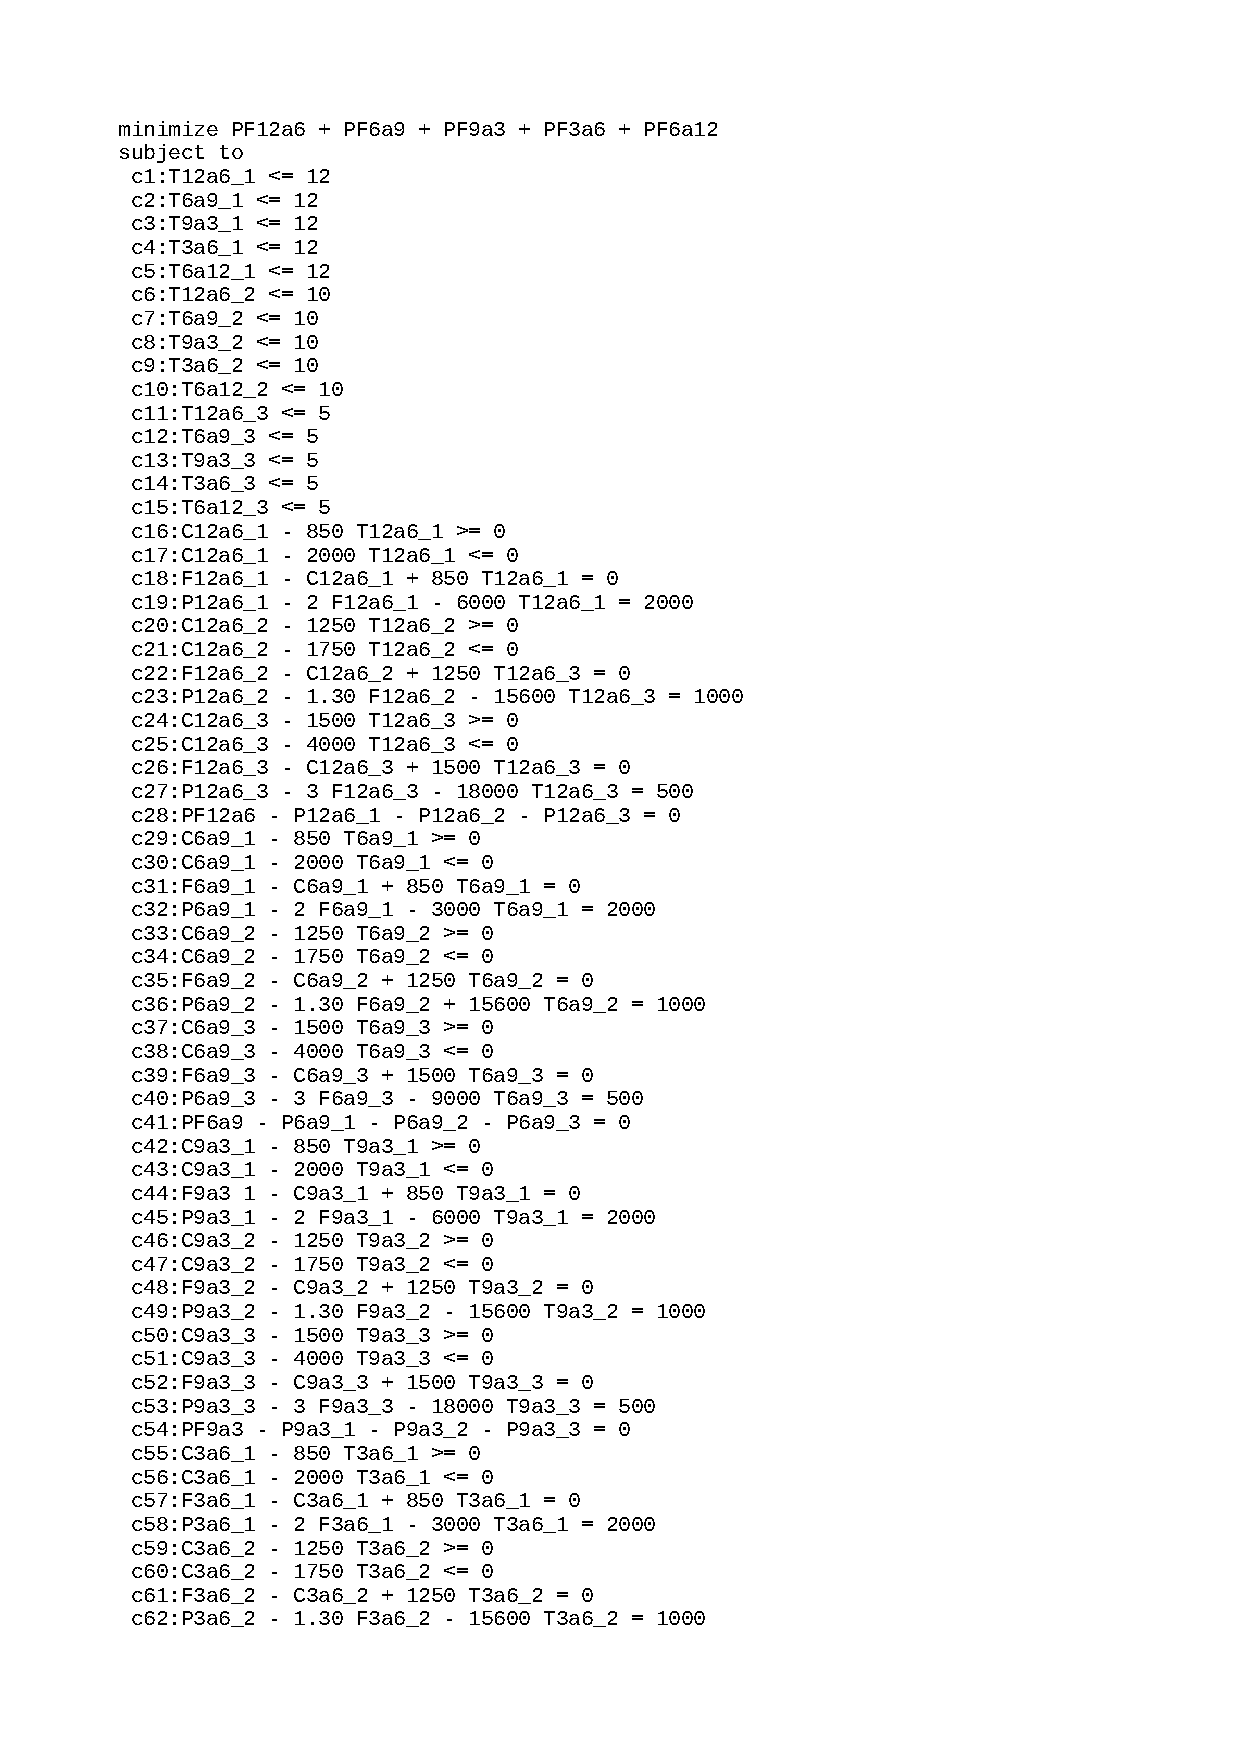
\includepdf[pages=1-2]{modelos/centralElectrica12-15}
\subsection{Solucion en CPLEX}

\paragraph{} ¿Qué generadores deberían estar trabajando en qué períodos del día para minimizar el costo total?
\begin{figure}[!h]
    \centering
    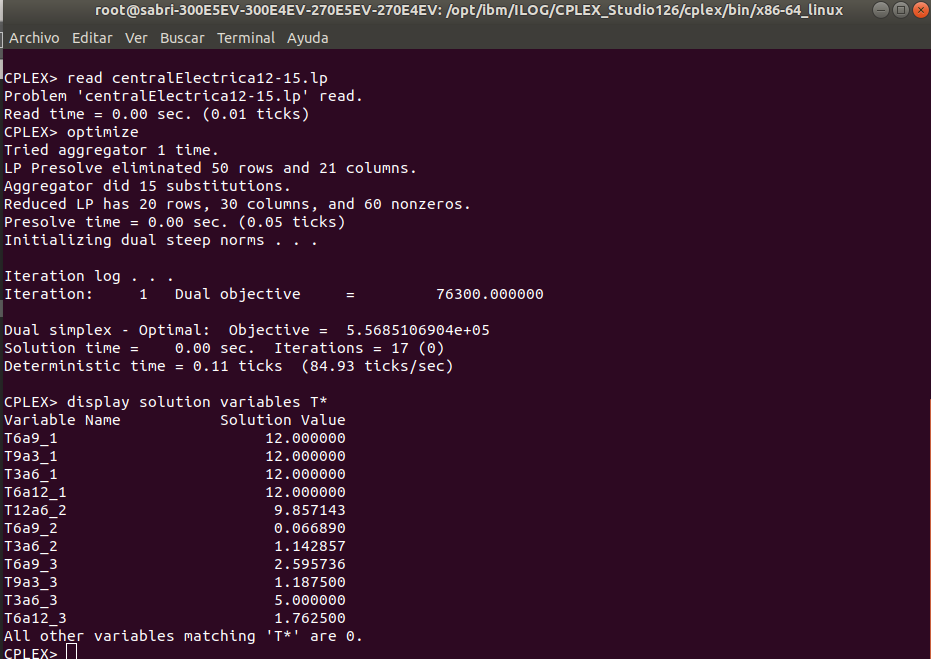
\includegraphics[scale=0.35]{modelos/SolutionCentralElectrica12-15Generadores.png}
    \caption{SolucionCentraElectricaGeneradores}
\end{figure}

\paragraph{} ¿Cuál es el costo marginal de producción de electricidad en cada período del día?; es decir, ¿qué aranceles deberían cobrarse?
\begin{figure}[!h]
    \centering
    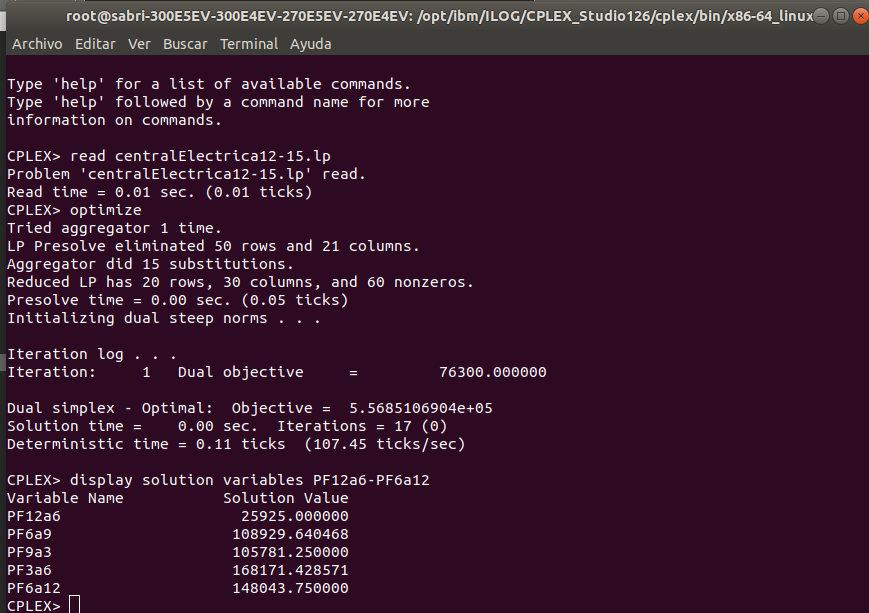
\includegraphics[scale=0.35]{modelos/SolutionCentralElectrica12-15PrecioPorRango.png}
    \caption{SolucionCentraElectricaGeneradores}
\end{figure}

\paragraph{} ¿Cuál sería el ahorro de reducir la garantía de reserva del aumento en la carga de hasta el 15\%? es decir, ¿cuánto cuesta esta garantía de reserva de suministro?\\
Modificamos estas restricciones:
\begin{equation}
C12a6_{1} + C12a6_{2} + C12a6_{3} \geq 17250
\end{equation}
\begin{equation}
C6a9_{1} + C6a9_{2} + C6a9_{3} \geq 34500
\end{equation}
\begin{equation}
C9a3_{1} + C9a3_{2} + C9a3_{3} \geq 28750
\end{equation}
\begin{equation}
C3a6_{1} + C3a6_{2} + C3a6_{3} \geq 46000
\end{equation}
\begin{equation}
C6a12_{1} + C6a12_{2} + C6a12_{3} \geq 31050
\end{equation}
\\ 
 por

\begin{equation}
C12a6_{1} + C12a6_{2} + C12a6_{3} \geq 15000
\end{equation}
\begin{equation}
C6a9_{1} + C6a9_{2} + C6a9_{3} \geq 30000
\end{equation}
\begin{equation}
C9a3_{1} + C9a3_{2} + C9a3_{3} \geq 25000
\end{equation}
\begin{equation}
C3a6_{1} + C3a6_{2} + C3a6_{3} \geq 40000
\end{equation}
\begin{equation}
C6a12_{1} + C6a12_{2} + C6a12_{3} \geq 27000
\end{equation}

\begin{figure}[!h]
    \centering
    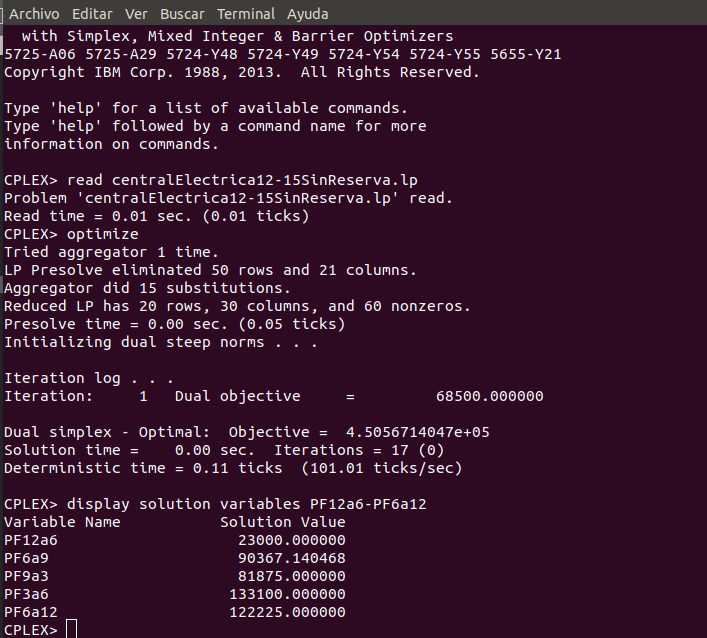
\includegraphics[scale=0.35]{modelos/SolutionCentralElectrica12-15PrecioPorRangoSinReserva.png}
    \caption{SolucionCentraElectricaGeneradores}
\end{figure}

\section{Energía hidroeléctrica}
\subsection{Enunciado 12.6}
\paragraph{} Esta es una extensión del problema de generación de energía. Además de los generadores térmicos, un depósito alimenta dos hidrogeneradores: en el tipo A y uno de tipo B. Cuando un hidrogenerador está funcionando, opera a un nivel fijo y la profundidad de deposito disminuye. Los costos asociados con cada hidrogenerador son un costo de puesta en marcha fijo y un costo de funcionamiento por hora. Las características de cada tipo de generador se muestran en la siguiente tabla:

\begin{center}
\begin{tabular}{ccccc}
\hline 
 & Operando a & Costo por & Reducción de la profundidad & Costo \\ 
 & nivel & hora & del embalse  por hora (m) & iniciales \\ 
\hline 
Hydro A & 900 MW & 90 & 0.31 & 1500 \\ 
\hline 
Hydro B & 1400 MW & 150 & 0.47 & 1200 \\ 
\hline 
\end{tabular} 
\end{center}

\paragraph{} Por razones medioambientales, el depósito debe mantenerse a una profundidad de entre 15 y 20 m. Además, a la medianoche de cada noche, el embalse debe ser de 16 m. profundo. Los generadores térmicos se pueden usar para bombear agua al depósito. Para aumentar el nivel del depósito en 1 m, requiere 3000 MWh de electricidad. Puede suponer que las precipitaciones no afectan el nivel del yacimiento.
\paragraph{} En cualquier momento, debe ser posible satisfacer un aumento en la demanda de electricidad de hasta 15\%. Esto puede lograrse mediante cualquier combinación de lo siguiente: encender un generador hidráulico (incluso si esto hiciera que la profundidad del depósito cayera por debajo de 15 m); utilizando la salida de un generador térmico, que se usa para bombear agua al depósito; y aumentar el nivel de operación de una generación térmica al máximo. Los generadores térmicos no se pueden encender instantáneamente para satisfacer la mayor demanda (aunque los generadores hidroeléctricos sí pueden).


\subsection{Modelo}
$\begin{array}{l}
D12a6:\mbox{profundidad del deposito desde 12 pm a 6 am}\\
D6a9:\mbox{profundidad del deposito desde 12 pm a 6 am}\\
D9a3:\mbox{profundidad del deposito desde 12 pm a 6 am}\\
D3a6:\mbox{profundidad del deposito desde 12 pm a 6 am}\\
D6a12:\mbox{profundidad del deposito desde 12 pm a 6 am}\\
H12a6_{i}:\mbox{se esta usando el hidrogenerador tipo i desde 12 pm a 6 am}\\
CH12a6_{i}:\mbox{costo total hidrogenerador tipo i desde 12 pm a 6 am}\\
H6a9_{i}:\mbox{se esta usando el hidrogenerador tipo i desde 6 am a 9 am}\\
CH6a9_{i}:\mbox{costo total hidrogenerador tipo i desde 6 am a 9 am}\\
H9a3_{i}:\mbox{se esta usando el hidrogenerador tipo i desde 9 am a 3 pm}\\
CH9a3_{i}:\mbox{costo total hidrogenerador tipo i desde 9 am a 3 pm}\\
H3a6_{i}:\mbox{se esta usando el hidrogenerador tipo i desde 3 pm a 6 pm}\\
CH3a6_{i}:\mbox{costo total hidrogenerador tipo i desde 3 pm a 6 pm}\\
H6a12_{i}:\mbox{se esta usando el hidrogenerador tipo i desde 6 pm a  12am}\\
CH6a12_{i}:\mbox{costo total hidrogenerador tipo i desde 6 pm a  12am}\\
\mbox{donde} \;\;\;\;\;\; i=A,B
\end{array}$
\\
\\
$$ \mbox{min } PF12a6 + PF6a9 + PF9a3 + PF3a6 + PF6a12 $$
\\ 
\\  
s.a\\
El deposito debe mantenerse a una profundidad entre 15 y 20 metros, ademas a la medianoche debe ser de al menos 16m.
\begin{equation}
D12a6 \geq 15 
\end{equation}
\begin{equation}
D12a6 \leq 20
\end{equation}
\begin{equation}
D6a9 \geq 15 
\end{equation}
\begin{equation}
D6a9 \leq 20
\end{equation}
\begin{equation}
D9a3 \geq 15 
\end{equation}
\begin{equation}
D9a3 \leq 20
\end{equation}
\begin{equation}
D3a6 \geq 15 
\end{equation}
\begin{equation}
D3a6 \leq 20
\end{equation}
\begin{equation}
D6a12 \geq 16  
\end{equation}
\begin{equation}
D6a12 \leq 20
\end{equation}
El desposito disminuye en metros si se utiliza un hidrogenerador
\begin{equation}
D12a6 - 0.31 (6 \times H12a6_{A}) - 0.47 (6 \times H12a6_{B}) \leq 20    
\end{equation}
\begin{equation}
D12a6 - 0.31 (6 \times H12a6_{A}) - 0.47 (6 \times H12a6_{B}) \geq 15    
\end{equation}
\begin{equation}
D6a9 - 0.31 (6 \times H6a9_{A}) - 0.47 (6 \times H6a9_{B}) \leq 20    
\end{equation}
\begin{equation}
D6a9 - 0.31 (6 \times H6a9_{A}) - 0.47 (6 \times H6a9_{B}) \geq 15    
\end{equation}
\begin{equation}
D9a3 - 0.31 (6 \times H9a3_{A}) - 0.47 (6 \times H9a3_{B}) \leq 20    
\end{equation}
\begin{equation}
D9a3 - 0.31 (6 \times H9a3_{A}) - 0.47 (6 \times H9a3_{B}) \geq 15    
\end{equation}
\begin{equation}
D3a6 - 0.31 (6 \times H3a6_{A}) - 0.47 (6 \times H3a6_{B}) \leq 20    
\end{equation}
\begin{equation}
D3a6 - 0.31 (6 \times H3a6_{A}) - 0.47 (6 \times H3a6_{B}) \geq 15    
\end{equation}
\begin{equation}
D6a12 - 0.31 (6 \times H6a12_{A}) - 0.47 (6 \times H6a12_{B}) \leq 20    
\end{equation}
\begin{equation}
D6a12 - 0.31 (6 \times H6a12_{A}) - 0.47 (6 \times H6a12_{B}) \geq 15    
\end{equation}
Indica si el hidrogenerador de tipo A o B se esta usando o no en ese rango horario
\begin{equation}
H12a6_{A} \geq 0
\end{equation}
\begin{equation}
H12a6_{B} \leq 1
\end{equation}
\begin{equation}
H6a9_{A} \geq 0 
\end{equation}
\begin{equation}
H6a9_{B} \leq 1
\end{equation}
\begin{equation}
H9a3_{A} \geq 0
\end{equation}
\begin{equation}
H9a3_{B} \leq 1
\end{equation}
\begin{equation}
H3a6_{A} \geq 0 
\end{equation}
\begin{equation}
H3a6_{B} \leq 1
\end{equation}
\begin{equation}
H6a12_{A} \geq 0 
\end{equation}
\begin{equation}
H6a12_{B} \leq 1
\end{equation}
\\
Costo de la energia proporcionada por el hidrogenerador en ese rango horario
\begin{equation}
CH12a6_{A} = (1500 + 90 \times 6) H12a6_{A}
\end{equation}
\begin{equation}
CH12a6_{B} = (1200 + 150 \times 6) H12a6_{B}  
\end{equation}
\begin{equation}
CH6a9_{A} = (1500 + 90 \times 3) H6a9_{A}
\end{equation}
\begin{equation}
CH6a9_{B} = (1200 + 150 \times 3) H6a9_{B} 
\end{equation}
\begin{equation}
CH9a3_{A} = (1500 + 90 \times 6) H9a3_{A}
\end{equation}
\begin{equation}
CH9a3_{B} = (1200 + 150 \times 6) H9a3_{B}  
\end{equation}
\begin{equation}
CH3a6_{A} = (1500 + 90 \times 3) H3a6_{A}
\end{equation}
\begin{equation}
CH3a6_{B} = (1200 + 150 \times 3) H3a6_{B} 
\end{equation}
\begin{equation}
CH6a12_{A} = (1500 + 90 \times 6) H6a12_{A}
\end{equation}
\begin{equation}
CH6a12_{B} = (1200 + 150 \times 6) H6a12_{B}
\end{equation}
    \newpage
    \section{Generación de energía}
\subsection{Enunciado 12.5}
\paragraph{} Varias centrales eléctricas se comprometen a cumplir las siguientes demandas de carga de electricidad durante un día:\\
\begin{center}
\begin{tabular}{cc}
\hline 
12 pm a 6 am & 15000 MW \\  
6 am a 9 am & 30000 MW \\  
9 am a 3 pm & 25000 MW \\  
3 pm a 6 pm & 40000 MW \\  
6 pm a 12 pm & 27000 MW \\ 
\hline 
\end{tabular} 
\end{center}

\paragraph{} Hay tres tipos de unidades generadoras disponibles: 12 de tipo 1, 10 de tipo 2 y cinco de tipo 3. Cada generador tiene que funcionar entre un nivel mínimo y un nivel máximo. Hay un costo por hora de funcionamiento de cada generador al nivel mínimo. Además, hay un costo adicional por hora por cada megavatio en el que se opera una unidad por encima del nivel mínimo. Iniciar un generador también implica un costo. Toda esta información se da en la tabla 12.6 (con costos en \pounds).
\begin{center}
\begin{tabular}{cccccc}
\hline 
 & Nivel & Nivel & Costo por  & Costo por hora & Costo \\ 
 & Minimo & Maximo & hora como & por megavatio &  \\ 
 &  &  & minimo & $>$ minimo &  \\ 
\hline 
Type 1 & 850 MW & 2000 MW & 1000 & 2 & 2000 \\ 
Type 2 & 1250 MW & 1750 MW & 2600 & 1.30 & 1000 \\ 
Type 3 & 1500 MW & 4000 MW & 3000 & 3 & 500 \\ 
\hline 
\end{tabular} 
\end{center}

\paragraph{} Además de cumplir con las demandas de carga estimadas, debe haber suficientes generadores trabajando en todo momento para que sea posible cumplir con un aumento en la carga de hasta 15\%. Este aumento tendría que lograrse ajustando la producción de los generadores que ya operan dentro de sus límites permitidos.

\paragraph{} ¿Qué generadores deberían estar trabajando en qué períodos del día para minimizar el costo total?

\paragraph{} ¿Cuál es el costo marginal de producción de electricidad en cada período del día?; es decir, ¿qué aranceles deberían cobrarse?

\paragraph{} ¿Cuál sería el ahorro de reducir la garantía de reserva del aumento en la carga de hasta el 15\%? es decir, ¿cuánto cuesta esta garantía de reserva de suministro?


\subsection{Modelo 12.5}
$\begin{array}{l}
T12a6_{i}:\mbox{\# de generadores tipo i usados desde 12 pm a 6 am}\\
C12a6_{i}:\mbox{\# de energia proporcionada por generador tipo i desde 12 pm a 6 am}\\
F12a6_{i}:\mbox{\# de energia con costo adicional generador tipo i desde 12 pm a 6 am}\\
P12a6_{i}:\mbox{costo total generador tipo i desde 12 pm a 6 am}\\
PF12a6:\mbox{costo total 12 pm a 6 am}\\
T6a9_{i}:\mbox{\# de generadores tipo i usados desde 6 am a 9 am}\\
C6a9_{i}:\mbox{\# de energia proporcionada por generador tipo i desde 6 am a 9 am}\\
F6a9_{i}:\mbox{\# de energia con costo adicional generador tipo i desde 6 am a 9 am}\\
P6a9_{i}:\mbox{costo total generador tipo i desde 6 am a 9 am}\\
PF6a9:\mbox{costo total 6 am a 9 am}\\
T9a3_{i}:\mbox{\# de generadores tipo i usados desde 9 am a 3 pm}\\
C9a3_{i}:\mbox{\# de energia proporcionada por generador tipo i desde 9 am a 3 pm}\\
F9a3_{i}:\mbox{\# de energia con costo adicional generador tipo i desde 9 am a 3 pm}\\
P9a3_{i}:\mbox{costo total generador tipo i desde 9 am a 3 pm}\\
PF9a3:\mbox{costo total 9 am a 3 pm}\\
T3a6_{i}:\mbox{\# de generadores tipo i usados desde 3 pm a 6 pm}\\
C3a6_{i}:\mbox{\# de energia proporcionada por generador tipo i desde 3 pm a 6 pm}\\
F3a6_{i}:\mbox{\# de energia con costo adicional generador tipo i desde 3 pm a 6 pm}\\
P3a6_{i}:\mbox{costo total generador tipo i desde 3 pm a 6 pm}\\
PF3a6:\mbox{costo total 3 pm a 6 pm}\\
T6a12_{i}:\mbox{\# de generadores tipo i usados desde 6 pm a 12 pm}\\
C6a12_{i}:\mbox{\# de energia proporcionada por generador tipo i desde 6 pm a 12 pm}\\
F6a12_{i}:\mbox{\# de energia con costo adicional generador tipo i desde 6 pm a 12 pm}\\
P6a12_{i}:\mbox{costo total generador tipo i desde 6 pm a 12 pm}\\
PF6a12:\mbox{costo total 6 pm a 12 pm}\\
\mbox{donde} \;\;\;\;\;\; i=1,2,3   
\end{array}$
\\
\\
$$ \mbox{min } PF12a6 + PF6a9 + PF9a3 + PF3a6 + PF6a12 $$
\\ 
\\  
s.a\\
\begin{equation}
T12a6_{1} \leq 12
\end{equation}
\begin{equation}
T6a9_{1} \leq 12
\end{equation}
\begin{equation}
T9a3_{1} \leq 12
\end{equation}
\begin{equation}
T3a6_{1} \leq 12
\end{equation}
\begin{equation}
T6a12_{1} \leq 12 
\end{equation}
\begin{equation}
T12a6_{2} \leq 10
\end{equation}
\begin{equation}
T6a9_{2} \leq 10
\end{equation}
\begin{equation}
T9a3_{2} \leq 10
\end{equation}
\begin{equation}
T3a6_{2} \leq 10
\end{equation}
\begin{equation}
T6a12_{2} \leq 10 
\end{equation}
\begin{equation}
T12a6_{3} \leq 5
\end{equation}
\begin{equation}
T6a9_{3} \leq 5
\end{equation}
\begin{equation}
T9a3_{3} \leq 5
\end{equation}
\begin{equation}
T3a6_{3} \leq 5
\end{equation}
\begin{equation}
T6a12_{3} \leq 5 
\end{equation}
%%%%%%%%%%%%%%%%%%%%%%%%%%%%%%%%Energia por horario 12 a 6
%la cantidad de energia debe estar en entre cantidad por el minimo y la cantidad por el maximo
%TIPO 1
\begin{equation}
C12a6_{1} \geq 850 T12a6_{1}
\end{equation}
\begin{equation}
C12a6_{1} \leq 2000 T12a6_{1}
\end{equation}
\begin{equation}
E12a6_{1} = C12a6_{1} - 850 T12a6_{1}
\end{equation}
\begin{equation}
P12a6_{1} = 2000 + 2 \; E12a6_{1} + 6 \; 1000 \; T12a6_{1}
\end{equation}
%TIPO 2
\begin{equation}
C12a6_{2} \geq 1250 T12a6_{2}
\end{equation}
\begin{equation}
C12a6_{2} \leq 1750 T12a6_{2}
\end{equation}
\begin{equation}
E12a6_{2} = C12a6_{2} - 1250 T12a6_{3}
\end{equation}
\begin{equation}
P12a6_{2} = 1000 + 1.30 \; E12a6_{2} + 6 \; 2600 \; T12a6_{3}
\end{equation}
%TIPO 3
\begin{equation}
C12a6_{3} \geq 1500 T12a6_{3}
\end{equation}
\begin{equation}
C12a6_{3} \leq 4000 T12a6_{3}
\end{equation}
\begin{equation}
E12a6_{3} = C12a6_{3} - 1500 T12a6_{3}
\end{equation}
\begin{equation}
P12a6_{3} = 500 + 3 \; E12a6_{3} + 6 \; 3000 \; T12a6_{3}
\end{equation}
\begin{equation}
PF12a6 = P12a6_{1} + P12a6_{2} + P12a6_{3} 
\end{equation}
%%%%%%%%%%%%%%%%%%%%%%%%%%%%%%%%Energia por horario 6 a 9
%la cantidad de energia debe estar en entre cantidad por el minimo y la cantidad por el maximo
%TIPO 1
\begin{equation}
C6a9_{1} \geq 850 T6a9_{1}
\end{equation}
\begin{equation}
C6a9_{1} \leq 2000 T6a9_{1}
\end{equation}
\begin{equation}
E6a9_{1} = C6a9_{1} - 850 T6a9_{1}
\end{equation}
\begin{equation}
P6a9_{1} = 2000 + 2 E6a9_{1} + 3 \; 1000 \; T6a9_{1}
\end{equation}
%TIPO 2
\begin{equation}
C6a9_{2} \geq 1250 T6a9_{2}
\end{equation}
\begin{equation}
C6a9_{2} \leq 1750 T6a9_{2}
\end{equation}
\begin{equation}
E6a9_{2} = C6a9_{2} - 1250 T6a9_{2}
\end{equation}
\begin{equation}
P6a9_{2} = 1000 + 1.30 E6a9_{2} + 3 \; 2600  \;T6a9_{2}
\end{equation}
%TIPO 3
\begin{equation}
C6a9_{3} \geq 1500 T6a9_{3}
\end{equation}
\begin{equation}
C6a9_{3} \leq 4000 T6a9_{3}
\end{equation}
\begin{equation}
E6a9_{3} = C6a9_{3} - 1500 T6a9_{3}
\end{equation}
\begin{equation}
P6a9_{3} = 500+ 3 \; E6a9_{3} + 3 \; 3000 \; T6a9_{3}
\end{equation}
\begin{equation}
PF6a9 = P6a9_{1} + P6a9_{2} + P6a9_{3}
\end{equation}
%%%%%%%%%%%%%%%%%%%%%%%%%%%%%%%%Energia por horario 9 a 3
%la cantidad de energia debe estar en entre cantidad por el minimo y la cantidad por el maximo
%TIPO 1
\begin{equation}
C9a3_{1} \geq 850 T9a3_{1}
\end{equation}
\begin{equation}
C9a3_{1} \leq 2000 T9a3_{1}
\end{equation}
\begin{equation}
E9a3_{1} = C9a3_{1} - 850 T9a3_{1}
\end{equation}
\begin{equation}
P9a3_{1} = 2000 + 2 \; E9a3_{1} + 6 \; 1000 \; T9a3_{1}
\end{equation}
%TIPO 2
\begin{equation}
C9a3_{2} \geq 1250 T9a3_{2}
\end{equation}
\begin{equation}
C9a3_{2} \leq 1750 T9a3_{2}
\end{equation}
\begin{equation}
E9a3_{2} = C9a3_{2} - 1250 T9a3_{2}
\end{equation}
\begin{equation}
P9a3_{2} = 1000 + 1.30 \; E9a3_{2} + 6 \; 2600 \; T9a3_{2}
\end{equation}
%TIPO 3
\begin{equation}
C9a3_{3} \geq 1500 T9a3_{3}
\end{equation}
\begin{equation}
C9a3_{3} \leq 4000 T9a3_{3}
\end{equation}
\begin{equation}
E9a3_{3} = C9a3_{3} - 1500 T9a3_{3}
\end{equation}
\begin{equation}
P9a3_{3} = 500 + 3 \; E9a3_{3} + 6 \; 3000 \; T9a3_{3}
\end{equation}
\begin{equation}
PF9a3 = P9a3_{1} + P9a3_{2} + P9a3_{3}
\end{equation}
%%%%%%%%%%%%%%%%%%%%%%%%%%%%%%%%Energia por horario 3a6
%la cantidad de energia debe estar en entre cantidad por el minimo y la cantidad por el maximo
%TIPO 1
\begin{equation}
C3a6_{1} \geq 850 T3a6_{1}
\end{equation}
\begin{equation}
C3a6_{1} \leq 2000 T3a6_{1}
\end{equation}
\begin{equation}
E3a6_{1} = C3a6_{1} - 850 T3a6_{1}
\end{equation}
\begin{equation}
P3a6_{1} = 2000 + 2 \; E3a6_{1} + 3 \; 1000 \; T3a6_{1}
\end{equation}
%TIPO 2
\begin{equation}
C3a6_{2} \geq 1250 T3a6_{2}
\end{equation}
\begin{equation}
C3a6_{2} \leq 1750 T3a6_{2}
\end{equation}
\begin{equation}
E3a6_{2} = C3a6_{2} - 1250 T3a6_{2}
\end{equation}
\begin{equation}
P3a6_{2} = 1000 + 1.30 \; E3a6_{2} + 3 \; 2600 \; T3a6_{2}
\end{equation}
%TIPO 3
\begin{equation}
C3a6_{3} \geq 1500 T3a6_{3}
\end{equation}
\begin{equation}
C3a6_{3} \leq 4000 T3a6_{3}
\end{equation}
\begin{equation}
E3a6_{3} = C3a6_{3} - 1500 T3a6_{3}
\end{equation}
\begin{equation}
P3a6_{3} = 500 + 3 \; E3a6_{3} + 3 \; 3000 \; T3a6_{3}
\end{equation}
\begin{equation}
PF3a6 = P3a6_{1} + P3a6_{2} + P3a6_{3}
\end{equation}
%%%%%%%%%%%%%%%%%%%%%%%%%%%%%%%%Energia por horario 6 a 12
%la cantidad de energia debe estar en entre cantidad por el minimo y la cantidad por el maximo
%TIPO 1
\begin{equation}
C6a12_{1} \geq 850 T6a12_{1}
\end{equation}
\begin{equation}
C6a12_{1} \leq 2000 T6a12_{1}
\end{equation}
\begin{equation}
E6a12_{1} = C6a12_{1} - 850 T6a12_{1}
\end{equation}
\begin{equation}
P6a12_{1} = 2000 + 2 \; E6a12_{1} + 6 \; 1000 \; T6a12_{1}
\end{equation}
%TIPO 2
\begin{equation}
C6a12_{2} \geq 1250 T6a12_{2}
\end{equation}
\begin{equation}
C6a12_{2} \leq 1750 T6a12_{2}
\end{equation}
\begin{equation}
E6a12_{2} = C6a12_{2} - 1250 T6a12_{2}
\end{equation}
\begin{equation}
P6a12_{2} = 1000 + 1.30 \; E6a12_{2} + 6 \; 2600 \; T6a12_{2}
\end{equation}
%TIPO 3
\begin{equation}
C6a12_{3} \geq 1500 T6a12_{3}
\end{equation}
\begin{equation}
C6a12_{3} \leq 4000 T6a12_{3}
\end{equation}
\begin{equation}
E6a12_{3} = C6a12_{3} - 1500 T6a12_{3}
\end{equation}
\begin{equation}
P6a12_{3} = 500 + 3 \; E6a12_{3} + 6 \; 3000 \; T6a12_{3}
\end{equation}
\begin{equation}
PF6a12 = P6a12_{1} + P6a12_{2} + P6a12_{3}
\end{equation}
%%%%%%%%%%%%%%%%%%%%%%%%%%%%%%%%%%%%%%%%%%%%
% Se deben cumplir con los requerimientos por horarios
%\begin{equation}
%C12a6_{1} + C12a6_{2} + C12a6_{3}  \geq 15000
%\end{equation}
\begin{equation}
C12a6_{1} + C12a6_{2} + C12a6_{3} \geq 17250
\end{equation}
%\begin{equation}
%C6a9_{1} + C6a9_{2} + C6a9_{3} \geq 30000
%\end{equation}
\begin{equation}
C6a9_{1} + C6a9_{2} + C6a9_{3} \geq 34500
\end{equation}
%\begin{equation}
%C9a3_{1} + C9a3_{2} + C9a3_{3} \geq 25000
%\end{equation}
\begin{equation}
C9a3_{1} + C9a3_{2} + C9a3_{3} \geq 28750
\end{equation}
%\begin{equation}
%C3a6_{1} + C3a6_{2} + C3a6_{3} \geq 40000
%\end{equation}
\begin{equation}
C3a6_{1} + C3a6_{2} + C3a6_{3} \geq 46000
\end{equation}
%\begin{equation}
%C6a12_{1} + C6a12_{2} + C6a12_{3} \geq 27000
%\end{equation}
\begin{equation}
C6a12_{1} + C6a12_{2} + C6a12_{3} \geq 31050
\end{equation}
\subsection{Modelo CPLEX 12-15}
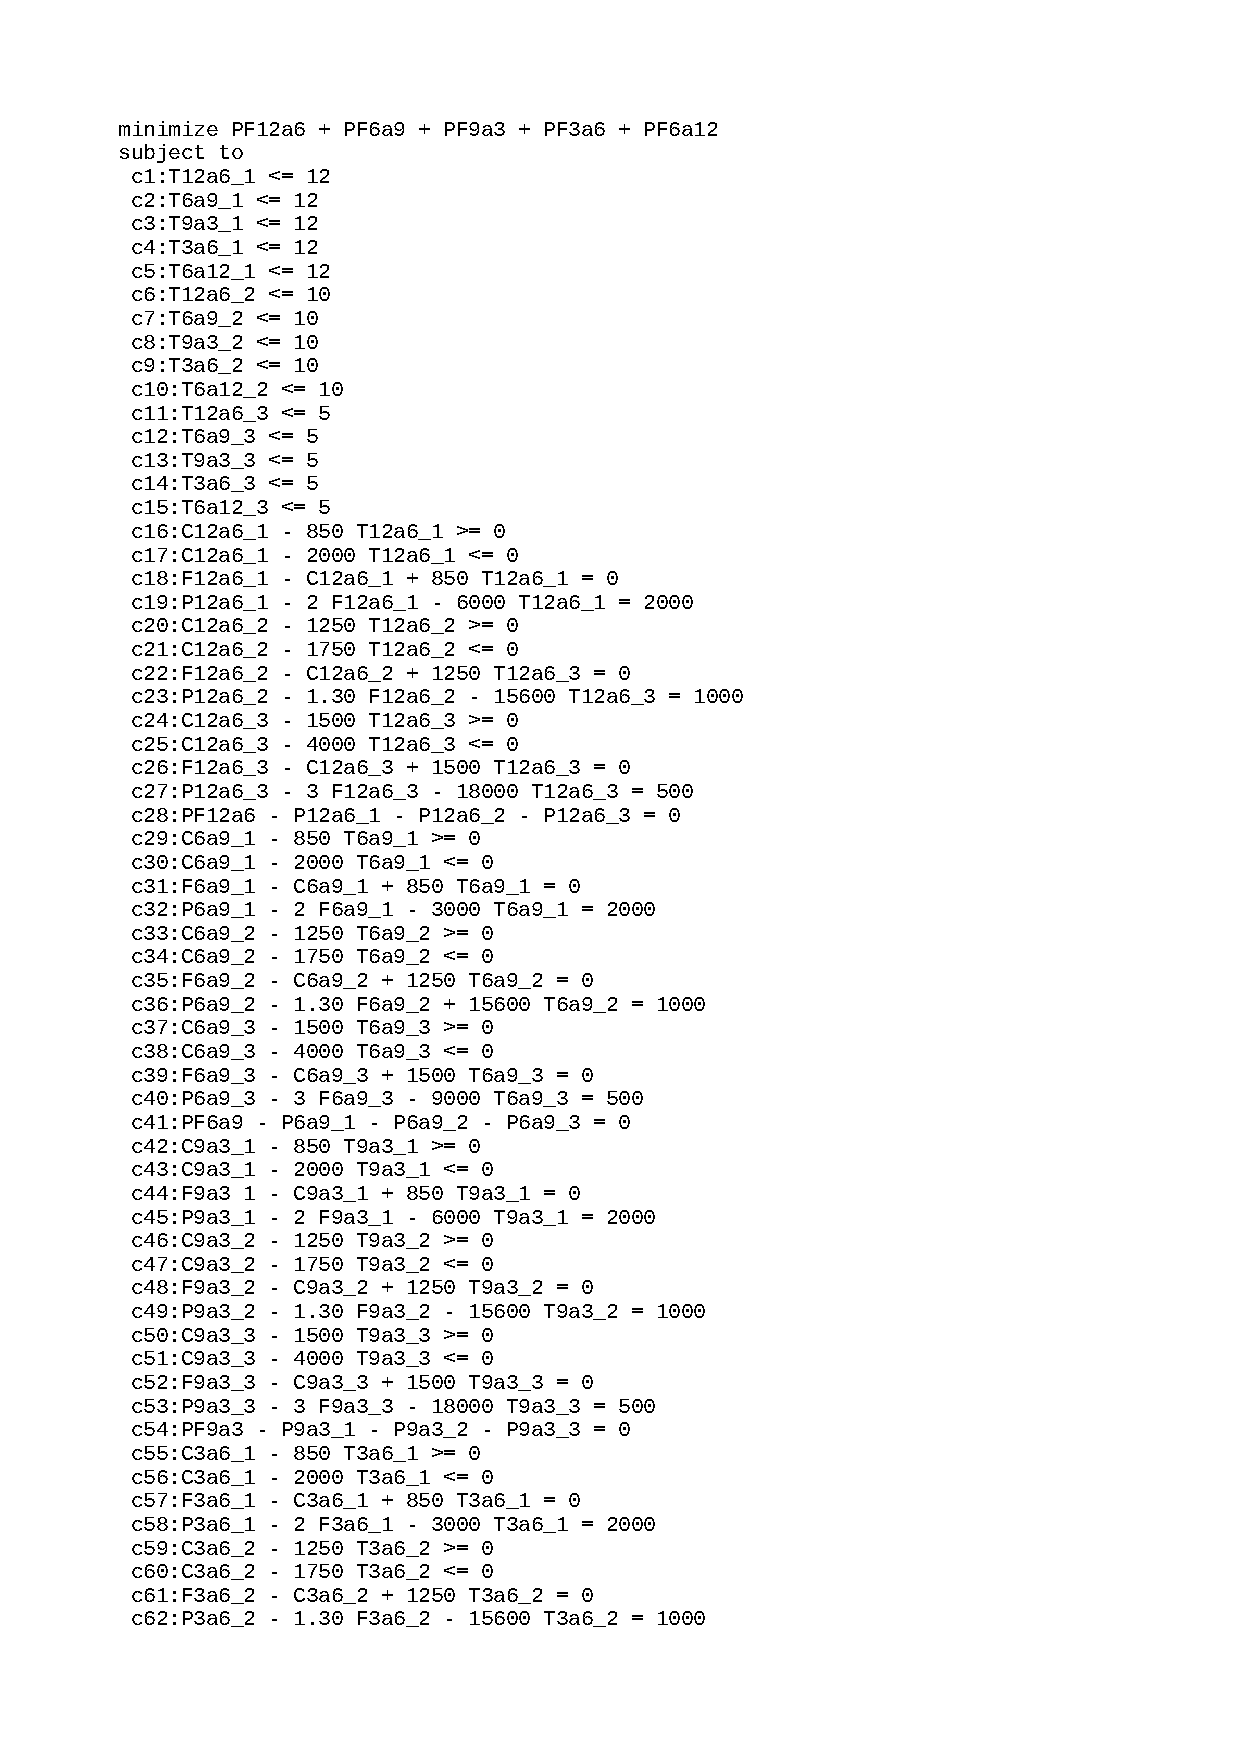
\includepdf[pages=1-2]{modelos/centralElectrica12-15}
\subsection{Solucion en CPLEX}

\paragraph{} ¿Qué generadores deberían estar trabajando en qué períodos del día para minimizar el costo total?
\begin{figure}[!h]
    \centering
    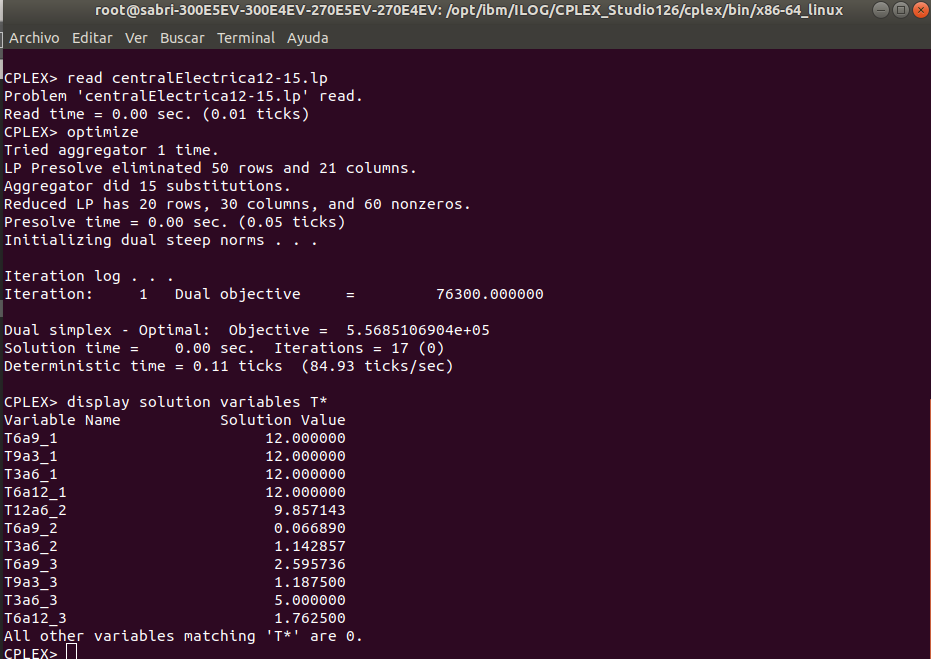
\includegraphics[scale=0.35]{modelos/SolutionCentralElectrica12-15Generadores.png}
    \caption{SolucionCentraElectricaGeneradores}
\end{figure}

\paragraph{} ¿Cuál es el costo marginal de producción de electricidad en cada período del día?; es decir, ¿qué aranceles deberían cobrarse?
\begin{figure}[!h]
    \centering
    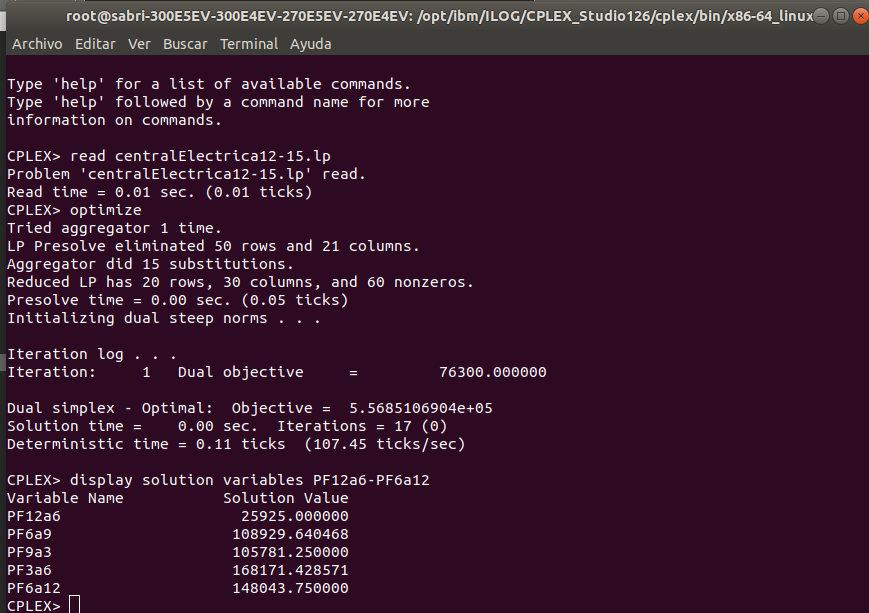
\includegraphics[scale=0.35]{modelos/SolutionCentralElectrica12-15PrecioPorRango.png}
    \caption{SolucionCentraElectricaGeneradores}
\end{figure}

\paragraph{} ¿Cuál sería el ahorro de reducir la garantía de reserva del aumento en la carga de hasta el 15\%? es decir, ¿cuánto cuesta esta garantía de reserva de suministro?\\
Modificamos estas restricciones:
\begin{equation}
C12a6_{1} + C12a6_{2} + C12a6_{3} \geq 17250
\end{equation}
\begin{equation}
C6a9_{1} + C6a9_{2} + C6a9_{3} \geq 34500
\end{equation}
\begin{equation}
C9a3_{1} + C9a3_{2} + C9a3_{3} \geq 28750
\end{equation}
\begin{equation}
C3a6_{1} + C3a6_{2} + C3a6_{3} \geq 46000
\end{equation}
\begin{equation}
C6a12_{1} + C6a12_{2} + C6a12_{3} \geq 31050
\end{equation}
\\ 
 por

\begin{equation}
C12a6_{1} + C12a6_{2} + C12a6_{3} \geq 15000
\end{equation}
\begin{equation}
C6a9_{1} + C6a9_{2} + C6a9_{3} \geq 30000
\end{equation}
\begin{equation}
C9a3_{1} + C9a3_{2} + C9a3_{3} \geq 25000
\end{equation}
\begin{equation}
C3a6_{1} + C3a6_{2} + C3a6_{3} \geq 40000
\end{equation}
\begin{equation}
C6a12_{1} + C6a12_{2} + C6a12_{3} \geq 27000
\end{equation}

\begin{figure}[!h]
    \centering
    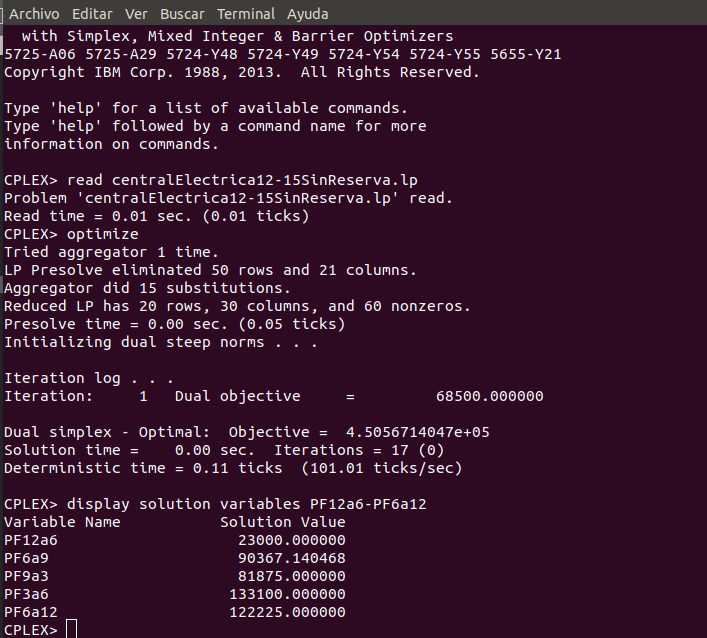
\includegraphics[scale=0.35]{modelos/SolutionCentralElectrica12-15PrecioPorRangoSinReserva.png}
    \caption{SolucionCentraElectricaGeneradores}
\end{figure}

\section{Energía hidroeléctrica}
\subsection{Enunciado 12.6}
\paragraph{} Esta es una extensión del problema de generación de energía. Además de los generadores térmicos, un depósito alimenta dos hidrogeneradores: en el tipo A y uno de tipo B. Cuando un hidrogenerador está funcionando, opera a un nivel fijo y la profundidad de deposito disminuye. Los costos asociados con cada hidrogenerador son un costo de puesta en marcha fijo y un costo de funcionamiento por hora. Las características de cada tipo de generador se muestran en la siguiente tabla:

\begin{center}
\begin{tabular}{ccccc}
\hline 
 & Operando a & Costo por & Reducción de la profundidad & Costo \\ 
 & nivel & hora & del embalse  por hora (m) & iniciales \\ 
\hline 
Hydro A & 900 MW & 90 & 0.31 & 1500 \\ 
\hline 
Hydro B & 1400 MW & 150 & 0.47 & 1200 \\ 
\hline 
\end{tabular} 
\end{center}

\paragraph{} Por razones medioambientales, el depósito debe mantenerse a una profundidad de entre 15 y 20 m. Además, a la medianoche de cada noche, el embalse debe ser de 16 m. profundo. Los generadores térmicos se pueden usar para bombear agua al depósito. Para aumentar el nivel del depósito en 1 m, requiere 3000 MWh de electricidad. Puede suponer que las precipitaciones no afectan el nivel del yacimiento.
\paragraph{} En cualquier momento, debe ser posible satisfacer un aumento en la demanda de electricidad de hasta 15\%. Esto puede lograrse mediante cualquier combinación de lo siguiente: encender un generador hidráulico (incluso si esto hiciera que la profundidad del depósito cayera por debajo de 15 m); utilizando la salida de un generador térmico, que se usa para bombear agua al depósito; y aumentar el nivel de operación de una generación térmica al máximo. Los generadores térmicos no se pueden encender instantáneamente para satisfacer la mayor demanda (aunque los generadores hidroeléctricos sí pueden).


\subsection{Modelo}
$\begin{array}{l}
D12a6:\mbox{profundidad del deposito desde 12 pm a 6 am}\\
D6a9:\mbox{profundidad del deposito desde 12 pm a 6 am}\\
D9a3:\mbox{profundidad del deposito desde 12 pm a 6 am}\\
D3a6:\mbox{profundidad del deposito desde 12 pm a 6 am}\\
D6a12:\mbox{profundidad del deposito desde 12 pm a 6 am}\\
H12a6_{i}:\mbox{se esta usando el hidrogenerador tipo i desde 12 pm a 6 am}\\
CH12a6_{i}:\mbox{costo total hidrogenerador tipo i desde 12 pm a 6 am}\\
H6a9_{i}:\mbox{se esta usando el hidrogenerador tipo i desde 6 am a 9 am}\\
CH6a9_{i}:\mbox{costo total hidrogenerador tipo i desde 6 am a 9 am}\\
H9a3_{i}:\mbox{se esta usando el hidrogenerador tipo i desde 9 am a 3 pm}\\
CH9a3_{i}:\mbox{costo total hidrogenerador tipo i desde 9 am a 3 pm}\\
H3a6_{i}:\mbox{se esta usando el hidrogenerador tipo i desde 3 pm a 6 pm}\\
CH3a6_{i}:\mbox{costo total hidrogenerador tipo i desde 3 pm a 6 pm}\\
H6a12_{i}:\mbox{se esta usando el hidrogenerador tipo i desde 6 pm a  12am}\\
CH6a12_{i}:\mbox{costo total hidrogenerador tipo i desde 6 pm a  12am}\\
\mbox{donde} \;\;\;\;\;\; i=A,B
\end{array}$
\\
\\
$$ \mbox{min } PF12a6 + PF6a9 + PF9a3 + PF3a6 + PF6a12 $$
\\ 
\\  
s.a\\
El deposito debe mantenerse a una profundidad entre 15 y 20 metros, ademas a la medianoche debe ser de al menos 16m.
\begin{equation}
D12a6 \geq 15 
\end{equation}
\begin{equation}
D12a6 \leq 20
\end{equation}
\begin{equation}
D6a9 \geq 15 
\end{equation}
\begin{equation}
D6a9 \leq 20
\end{equation}
\begin{equation}
D9a3 \geq 15 
\end{equation}
\begin{equation}
D9a3 \leq 20
\end{equation}
\begin{equation}
D3a6 \geq 15 
\end{equation}
\begin{equation}
D3a6 \leq 20
\end{equation}
\begin{equation}
D6a12 \geq 16  
\end{equation}
\begin{equation}
D6a12 \leq 20
\end{equation}
El desposito disminuye en metros si se utiliza un hidrogenerador
\begin{equation}
D12a6 - 0.31 (6 \times H12a6_{A}) - 0.47 (6 \times H12a6_{B}) \leq 20    
\end{equation}
\begin{equation}
D12a6 - 0.31 (6 \times H12a6_{A}) - 0.47 (6 \times H12a6_{B}) \geq 15    
\end{equation}
\begin{equation}
D6a9 - 0.31 (6 \times H6a9_{A}) - 0.47 (6 \times H6a9_{B}) \leq 20    
\end{equation}
\begin{equation}
D6a9 - 0.31 (6 \times H6a9_{A}) - 0.47 (6 \times H6a9_{B}) \geq 15    
\end{equation}
\begin{equation}
D9a3 - 0.31 (6 \times H9a3_{A}) - 0.47 (6 \times H9a3_{B}) \leq 20    
\end{equation}
\begin{equation}
D9a3 - 0.31 (6 \times H9a3_{A}) - 0.47 (6 \times H9a3_{B}) \geq 15    
\end{equation}
\begin{equation}
D3a6 - 0.31 (6 \times H3a6_{A}) - 0.47 (6 \times H3a6_{B}) \leq 20    
\end{equation}
\begin{equation}
D3a6 - 0.31 (6 \times H3a6_{A}) - 0.47 (6 \times H3a6_{B}) \geq 15    
\end{equation}
\begin{equation}
D6a12 - 0.31 (6 \times H6a12_{A}) - 0.47 (6 \times H6a12_{B}) \leq 20    
\end{equation}
\begin{equation}
D6a12 - 0.31 (6 \times H6a12_{A}) - 0.47 (6 \times H6a12_{B}) \geq 15    
\end{equation}
Indica si el hidrogenerador de tipo A o B se esta usando o no en ese rango horario
\begin{equation}
H12a6_{A} \geq 0
\end{equation}
\begin{equation}
H12a6_{B} \leq 1
\end{equation}
\begin{equation}
H6a9_{A} \geq 0 
\end{equation}
\begin{equation}
H6a9_{B} \leq 1
\end{equation}
\begin{equation}
H9a3_{A} \geq 0
\end{equation}
\begin{equation}
H9a3_{B} \leq 1
\end{equation}
\begin{equation}
H3a6_{A} \geq 0 
\end{equation}
\begin{equation}
H3a6_{B} \leq 1
\end{equation}
\begin{equation}
H6a12_{A} \geq 0 
\end{equation}
\begin{equation}
H6a12_{B} \leq 1
\end{equation}
\\
Costo de la energia proporcionada por el hidrogenerador en ese rango horario
\begin{equation}
CH12a6_{A} = (1500 + 90 \times 6) H12a6_{A}
\end{equation}
\begin{equation}
CH12a6_{B} = (1200 + 150 \times 6) H12a6_{B}  
\end{equation}
\begin{equation}
CH6a9_{A} = (1500 + 90 \times 3) H6a9_{A}
\end{equation}
\begin{equation}
CH6a9_{B} = (1200 + 150 \times 3) H6a9_{B} 
\end{equation}
\begin{equation}
CH9a3_{A} = (1500 + 90 \times 6) H9a3_{A}
\end{equation}
\begin{equation}
CH9a3_{B} = (1200 + 150 \times 6) H9a3_{B}  
\end{equation}
\begin{equation}
CH3a6_{A} = (1500 + 90 \times 3) H3a6_{A}
\end{equation}
\begin{equation}
CH3a6_{B} = (1200 + 150 \times 3) H3a6_{B} 
\end{equation}
\begin{equation}
CH6a12_{A} = (1500 + 90 \times 6) H6a12_{A}
\end{equation}
\begin{equation}
CH6a12_{B} = (1200 + 150 \times 6) H6a12_{B}
\end{equation}
    \newpage
    \section{Colección de leche}
\subsection{Enunciado}
\paragraph{} Una pequeña empresa de procesamiento de leche se ha comprometido a recolectar leche de 20 granjas y llevarla al depósito para su procesamiento. La compañía tiene un camión cisterna con capacidad para transportar 80000 litros de leche. Once de las granjas son pequeñas y solo necesitan una recolección cada dos días. Las otras nueve granjas necesitan una colección todos los días. Las posiciones de las granjas en relación con el depósito (numeradas 1) junto con sus requisitos de recolección se muestran en la siguiente tabla:

\begin{center}
\begin{tabular}{ccccc}
\hline 
Granja & Posicion & 10 miles & Recolección  & Requisito de \\ 
 &  &  & frecuencia & recolección \\ 
 &  &  &  & (10001) \\ 
\hline 
1 (deposito) & 0 & 0 & - & - \\ 
2 & -3 & 3 & Cada día & 5 \\ 
3 & 1 & 11 & Cada día & 4 \\ 
4 & 4 & 7 & Cada día & 3 \\ 
5 & -5 & 9 & Cada día & 6 \\ 
6 & -5 & -2 & Cada día & 7 \\ 
7 & -4 & -7 & Cada día & 3 \\ 
8 & 6 & 0 & Cada día & 4 \\ 
9 & 3 & -6 & Cada día & 6 \\ 
10 & -1 & -3 & Cada día & 5 \\ 
11 & 0 & -6 & Cualquier otro día & 4 \\ 
12 & 6 & 4 & Cualquier otro día & 7 \\ 
13 & 2 & 5 & Cualquier otro día & 3 \\ 
14 & -2 & 8 & Cualquier otro día & 4 \\ 
15 & 6 & 10 & Cualquier otro día & 5 \\ 
16 & 1 & 8 & Cualquier otro día & 6 \\ 
17 & -3 & 1 & Cualquier otro día & 8 \\ 
18 & -6 & 5 & Cualquier otro día & 5 \\ 
19 & 2 & 9 & Cualquier otro día & 7 \\ 
20 & -6 & -5 & Cualquier otro día & 6 \\ 
21 & 5 & -4 & Cualquier otro día & 6 \\ 
\hline 
\end{tabular} 
\end{center}
\paragraph{} Encuentre la ruta óptima para el camión cisterna cada día, teniendo en cuenta que tiene que (i) visitar todas las granjas \' todos los días\', (ii) visitar algunas de las granjas \' cada dos días\' y (iii) trabajar dentro de es capacidad. En días alternos, debe volver a visitar las granjas \' todos los días\' y también visitar las granjas \' cada dos días \' no visitadas el día anterior.
\paragraph{} Para mayor comodidad, se proporciona un mapa del área considerada en la figura 12.7.
%\section{Bibliografia}
\end{document}
